\documentclass[aspectratio=169,11pt]{beamer}

\ifdefined\moduleid
  \expandafter\includeonlylecture\expandafter{\moduleid}
\fi

\usepackage[T1]{fontenc}
\usepackage[utf8]{inputenc}
\usepackage{lmodern}
\usepackage{booktabs}
\usepackage{array}
\usepackage{listings}
\usepackage{graphicx}
\usepackage{tikz}
\usetikzlibrary{arrows.meta,calc,fit,positioning,shapes.geometric}

% ---------------------------------------------------------------------------
% Editable course metadata
% ---------------------------------------------------------------------------
\newcommand{\coursename}{Process Mining}
\newcommand{\coursesubtitle}{From Event Data to Process Insight}
\newcommand{\instructor}{Sylvio Barbon Junior}
\newcommand{\institution}{Institution / Program}

% ---------------------------------------------------------------------------
% Visual language
% ---------------------------------------------------------------------------
\definecolor{Ink}{HTML}{14213D}
\definecolor{DeepInk}{HTML}{0B132B}
\definecolor{Paper}{HTML}{F7F3EA}
\definecolor{Coral}{HTML}{F05D5E}
\definecolor{Teal}{HTML}{0F8B8D}
\definecolor{Gold}{HTML}{F2B134}
\definecolor{Mist}{HTML}{DCE8E8}
\definecolor{SoftGray}{HTML}{6B7280}
\definecolor{CodeBg}{HTML}{EEF2F3}

\setbeamercolor{normal text}{fg=Ink,bg=Paper}
\setbeamercolor{structure}{fg=Teal}
\setbeamercolor{frametitle}{fg=Ink,bg=Paper}
\setbeamercolor{title}{fg=Paper}
\setbeamercolor{subtitle}{fg=Mist}
\setbeamercolor{block title}{fg=Paper,bg=Ink}
\setbeamercolor{block body}{fg=Ink,bg=Mist!55!Paper}
\setbeamercolor{alerted text}{fg=Coral}
\setbeamercolor{itemize item}{fg=Coral}
\setbeamercolor{itemize subitem}{fg=Teal}

\setbeamertemplate{navigation symbols}{}
\setbeamertemplate{itemize item}{\raise0.15ex\hbox{\color{Coral}\small$\blacktriangleright$}}
\setbeamertemplate{itemize subitem}{\raise0.15ex\hbox{\color{Teal}\scriptsize$\bullet$}}
\setbeamertemplate{blocks}[rounded][shadow=false]
\setbeamertemplate{frametitle}{
  \vspace{0.35cm}
  \usebeamerfont{frametitle}\insertframetitle\par
  \vspace{-0.05cm}
  {\color{Coral}\rule{1.25cm}{1.8pt}}
}
\setbeamertemplate{footline}{
  \leavevmode
  \hbox{%
    \begin{beamercolorbox}[wd=.78\paperwidth,ht=2.8ex,dp=1.2ex,leftskip=.55cm]{normal text}
      \scriptsize\color{SoftGray}\coursename\hspace{0.5em}/\hspace{0.5em}\insertsectionhead
    \end{beamercolorbox}%
    \begin{beamercolorbox}[wd=.22\paperwidth,ht=2.8ex,dp=1.2ex,rightskip=.55cm plus1fil]{normal text}
      \scriptsize\color{SoftGray}\insertframenumber\,/\,\inserttotalframenumber
    \end{beamercolorbox}%
  }
}

\setbeamerfont{title}{size=\fontsize{28}{31}\selectfont,series=\bfseries}
\setbeamerfont{subtitle}{size=\large}
\setbeamerfont{frametitle}{size=\Large,series=\bfseries}
\setbeamerfont{section title}{size=\fontsize{26}{29}\selectfont,series=\bfseries}

\lstdefinestyle{python}{
  language=Python,
  basicstyle=\ttfamily\scriptsize,
  keywordstyle=\color{Teal}\bfseries,
  stringstyle=\color{Coral},
  commentstyle=\color{SoftGray}\itshape,
  backgroundcolor=\color{CodeBg},
  frame=single,
  rulecolor=\color{Mist},
  showstringspaces=false,
  breaklines=true,
  columns=fullflexible,
  keepspaces=true,
  xleftmargin=0.4em,
  framexleftmargin=0.4em
}

\tikzset{
  activity/.style={
    rounded corners=2pt, draw=Ink, thick, fill=Paper,
    minimum width=1.65cm, minimum height=0.72cm, align=center
  },
  event/.style={
    circle, fill=Coral, text=Paper, minimum size=0.66cm,
    inner sep=0pt, font=\scriptsize\bfseries
  },
  object/.style={
    rounded corners=2pt, draw=Teal, thick, fill=Mist,
    minimum width=1.35cm, minimum height=0.62cm, align=center
  },
  flow/.style={-{Stealth[length=2.2mm]}, thick, draw=Ink},
  softflow/.style={-{Stealth[length=2mm]}, thick, draw=SoftGray},
  accentflow/.style={-{Stealth[length=2.2mm]}, very thick, draw=Coral}
}

\newcommand{\keyidea}[1]{%
  \begin{beamercolorbox}[rounded=true,sep=0.65em]{block body}
    \textbf{\color{Teal}Key idea}\quad #1
  \end{beamercolorbox}
}

\newcommand{\promptbox}[1]{%
  \begin{beamercolorbox}[rounded=true,sep=0.65em]{block body}
    \textbf{\color{Coral}Discuss}\quad #1
  \end{beamercolorbox}
}

\newcommand{\unitdivider}[3]{%
  \begin{frame}[plain]
    \begin{tikzpicture}[remember picture,overlay]
      \fill[DeepInk] (current page.south west) rectangle (current page.north east);
      \fill[Coral] (current page.south west) rectangle
        ([xshift=0.18\paperwidth]current page.north west);
      \draw[Teal,line width=6pt]
        ([xshift=0.18\paperwidth,yshift=-1.2cm]current page.north west) --
        ([xshift=0.92\paperwidth,yshift=-1.2cm]current page.north west);
      \node[anchor=west,text=Paper,font=\fontsize{42}{42}\selectfont\bfseries]
        at ([xshift=0.055\paperwidth]current page.west) {#1};
      \node[anchor=west,text=Paper,text width=0.66\paperwidth,
        font=\fontsize{24}{28}\selectfont\bfseries]
        at ([xshift=0.23\paperwidth,yshift=0.55cm]current page.west) {#2};
      \node[anchor=west,text=Mist,text width=0.66\paperwidth,font=\large]
        at ([xshift=0.23\paperwidth,yshift=-1.05cm]current page.west) {#3};
    \end{tikzpicture}
  \end{frame}
}

\title{\coursename}
\subtitle{\coursesubtitle}
\author{\instructor}
\institute{\institution}
\date{}

\begin{document}

% ===========================================================================
% Opening
% ===========================================================================
\lecture{Course overview}{00}
\begin{frame}[plain]
  \begin{tikzpicture}[remember picture,overlay]
    \fill[DeepInk] (current page.south west) rectangle (current page.north east);
    \fill[Teal] ([xshift=0.72\paperwidth]current page.south west)
      rectangle (current page.north east);
    \fill[Coral]
      ([xshift=0.72\paperwidth,yshift=0.63\paperheight]current page.south west)
      rectangle (current page.north east);

    \node[anchor=west,text=Paper,text width=0.61\paperwidth]
      at ([xshift=0.07\paperwidth,yshift=0.10\paperheight]current page.west)
      {\usebeamerfont{title}\inserttitle};
    \node[anchor=west,text=Mist,text width=0.58\paperwidth]
      at ([xshift=0.07\paperwidth,yshift=-0.05\paperheight]current page.west)
      {\usebeamerfont{subtitle}\insertsubtitle};
    \node[anchor=west,text=Paper!75,font=\small]
      at ([xshift=0.07\paperwidth,yshift=-0.25\paperheight]current page.west)
      {\insertauthor\quad|\quad\insertinstitute};

    \node[event] (e1) at ([xshift=0.78\paperwidth,yshift=0.18\paperheight]current page.south west) {1};
    \node[event,fill=Gold,text=Ink] (e2) at ([xshift=0.88\paperwidth,yshift=0.30\paperheight]current page.south west) {2};
    \node[event,fill=Paper,text=Ink] (e3) at ([xshift=0.80\paperwidth,yshift=0.45\paperheight]current page.south west) {3};
    \draw[flow,draw=Paper] (e1) -- (e2);
    \draw[flow,draw=Paper] (e2) -- (e3);

    \node[anchor=north east,fill=Paper,inner sep=3pt,rounded corners=2pt]
      (qr) at ([xshift=-0.35cm,yshift=-0.35cm]current page.north east)
      {
\includegraphics[width=1.9cm]{../../assets/slides/repo-qrcode.png}};
    \node[anchor=north,font=\tiny,text=Paper,text width=2.3cm,align=center]
      at ([yshift=-0.1cm]qr.south)
      {Course repository};
  \end{tikzpicture}
\end{frame}

\section{Course map}

\begin{frame}{What this course is really about}
  \begin{columns}[T,onlytextwidth]
    \column{0.31\textwidth}
      \begin{block}{Observe}
        Turn operational records into trustworthy event data.
      \end{block}
    \column{0.31\textwidth}
      \begin{block}{Explain}
        Reveal paths, choices, delays, rework, and deviations.
      \end{block}
    \column{0.31\textwidth}
      \begin{block}{Improve}
        Convert evidence into a testable process intervention.
      \end{block}
  \end{columns}
  \vspace{0.55cm}
  \keyidea{Process mining connects \alert{data} to \alert{process behavior}.
  The diagram is not the result; the defensible explanation is.}
  \vspace{0.3cm}
  \begin{center}
    \small\color{SoftGray}Course repository:\quad
    \href{https://github.com/sbarbonjr/process_mining_course}{\color{Teal}\texttt{github.com/sbarbonjr/process\_mining\_course}}
  \end{center}
\end{frame}

\begin{frame}{The learning journey}
  \centering
  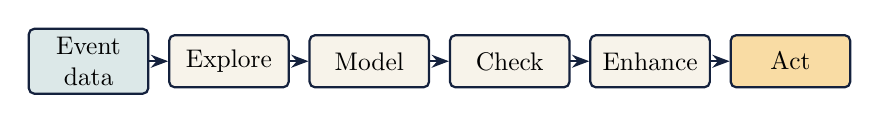
\begin{tikzpicture}[node distance=0.26cm and 0.26cm,scale=0.92,transform shape]
    \node[activity,fill=Mist] (a) {Event\\data};
    \node[activity,right=of a] (b) {Explore};
    \node[activity,right=of b] (c) {Model};
    \node[activity,right=of c] (d) {Check};
    \node[activity,right=of d] (e) {Enhance};
    \node[activity,right=of e,fill=Gold!45] (f) {Act};
    \draw[flow] (a)--(b);
    \draw[flow] (b)--(c);
    \draw[flow] (c)--(d);
    \draw[flow] (d)--(e);
    \draw[flow] (e)--(f);
  \end{tikzpicture}

  \vspace{0.65cm}
  \begin{columns}[T,onlytextwidth]
    \column{0.48\textwidth}
      \textbf{Foundation}
      \begin{itemize}
        \item Process questions and event semantics
        \item Data quality and exploratory analysis
        \item Behavioral models and discovery
      \end{itemize}
    \column{0.48\textwidth}
      \textbf{Application}
      \begin{itemize}
        \item Model quality and conformance
        \item Performance and organizational views
        \item Object-centric analysis and delivery
      \end{itemize}
  \end{columns}
\end{frame}

\begin{frame}{Course operating model}
  \begin{columns}[T,onlytextwidth]
    \column{0.52\textwidth}
      \textbf{Each unit combines}
      \begin{itemize}
        \item Concepts and visual intuition
        \item A worked event-log example
        \item A PM4Py laboratory
        \item A short interpretation challenge
      \end{itemize}
      \vspace{0.3cm}
      \textbf{Core tools}\\
      Python, pandas, PM4Py, Jupyter, Graphviz, Git
    \column{0.43\textwidth}
      \begin{block}{Assessment}
        \begin{tabular}{@{}lr@{}}
          Labs & 30\%\\
          Concept checks & 20\%\\
          Capstone analysis & 35\%\\
          Presentation & 15\%
        \end{tabular}
      \end{block}
      \promptbox{What process do you encounter every week that leaves a digital trace?}
  \end{columns}
\end{frame}

% ===========================================================================
% Unit 1
% ===========================================================================
\lecture{Process Thinking and Process Mining}{01}
\section{Process thinking}
\unitdivider{01}{Process Thinking and Process Mining}
  {Start with the operational question, not the algorithm.}

\begin{frame}{A process is behavior over time}
  \begin{columns}[T,onlytextwidth]
    \column{0.54\textwidth}
      A process consists of:
      \begin{itemize}
        \item \textbf{Cases}: process instances
        \item \textbf{Activities}: meaningful steps
        \item \textbf{Events}: recorded activity executions
        \item \textbf{Resources}: people or systems involved
        \item \textbf{Outcomes}: time, cost, quality, compliance
      \end{itemize}
    \column{0.41\textwidth}
      \centering
      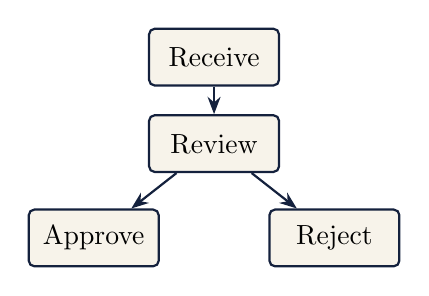
\begin{tikzpicture}[node distance=0.35cm]
        \node[activity] (a) {Receive};
        \node[activity,below=of a] (b) {Review};
        \node[activity,below left=0.45cm and -0.15cm of b] (c) {Approve};
        \node[activity,below right=0.45cm and -0.15cm of b] (d) {Reject};
        \draw[flow] (a)--(b);
        \draw[flow] (b)--(c);
        \draw[flow] (b)--(d);
      \end{tikzpicture}
  \end{columns}
  \vspace{0.35cm}
  \keyidea{A process model is a claim about possible behavior. An event log is
  evidence of observed behavior.}
\end{frame}

\begin{frame}{Four questions, four branches}
  \centering
  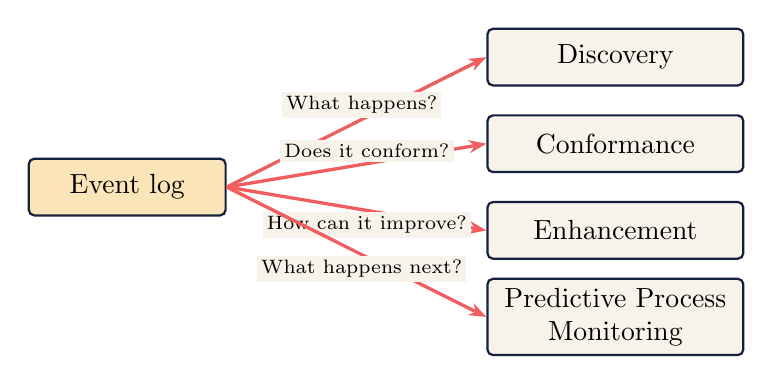
\begin{tikzpicture}[x=1cm,y=1cm]
    \node[activity,fill=Gold!35,minimum width=2.5cm] (log) at (-3.7,0) {Event log};
    \node[activity,minimum width=3.25cm] (disc) at (2.5,1.65) {Discovery};
    \node[activity,minimum width=3.25cm] (conf) at (2.5,0.55) {Conformance};
    \node[activity,minimum width=3.25cm] (enh) at (2.5,-0.55) {Enhancement};
    \node[activity,minimum width=3.25cm] (pred) at (2.5,-1.65)
      {Predictive Process\\Monitoring};

    \draw[accentflow] (log.east) -- node[pos=0.52,above,fill=Paper,
      inner sep=1.5pt,font=\scriptsize]{What happens?} (disc.west);
    \draw[accentflow] (log.east) -- node[pos=0.54,above,fill=Paper,
      inner sep=1.5pt,font=\scriptsize]{Does it conform?} (conf.west);
    \draw[accentflow] (log.east) -- node[pos=0.54,below,fill=Paper,
      inner sep=1.5pt,font=\scriptsize]{How can it improve?} (enh.west);
    \draw[accentflow] (log.east) -- node[pos=0.52,below,fill=Paper,
      inner sep=1.5pt,font=\scriptsize]{What happens next?} (pred.west);
  \end{tikzpicture}
  \vspace{0.3cm}
  \begin{columns}[T,onlytextwidth]
    \column{0.23\textwidth}\textbf{Discover}\\Reveal actual behavior.
    \column{0.23\textwidth}\textbf{Check}\\Compare log and model.
    \column{0.23\textwidth}\textbf{Enhance}\\Add time, cost, or decisions.
    \column{0.23\textwidth}\textbf{Predict}\\Anticipate outcomes, delays, and risks.
  \end{columns}
\end{frame}

\begin{frame}{Process mining is not a dashboard}
  \begin{tabular}{@{}>{\bfseries}p{0.20\textwidth}p{0.34\textwidth}p{0.36\textwidth}@{}}
    \toprule
    & Typical analytics & Process mining\\
    \midrule
    Unit & Rows and aggregates & Cases and ordered events\\
    Question & How many? & How did work unfold?\\
    Structure & Usually tabular & Sequential, concurrent, cyclic\\
    Output & KPI or prediction & Behavior, deviation, performance\\
    Risk & Missed context & Misleading case/event semantics\\
    \bottomrule
  \end{tabular}
  \vspace{0.5cm}
  \promptbox{A delivery KPI worsened. What sequence-level questions would you ask
  before recommending a change?}
\end{frame}

\begin{frame}{Frame a useful analysis}
  \begin{enumerate}
    \item \textbf{Decision}: What decision should this analysis support?
    \item \textbf{Scope}: Where does the process begin and end?
    \item \textbf{Case}: What is one process instance?
    \item \textbf{Evidence}: Which systems record relevant events?
    \item \textbf{Success}: Which behavior or outcome should change?
  \end{enumerate}
  \vspace{0.35cm}
  \begin{block}{Example}
    ``Why are some orders late?'' becomes: ``Which paths, handovers, and waiting
    periods distinguish orders delivered after the five-day target?''
  \end{block}
\end{frame}

% ===========================================================================
% Unit 2
% ===========================================================================
\lecture{Event Data and Event-Log Semantics}{02}
\section{Event-log semantics}
\unitdivider{02}{Event Data and Event-Log Semantics}
  {The quality of the analysis begins with the meaning of an event.}

\begin{frame}{The minimum viable event log}
  \small
  \begin{tabular}{@{}lllll@{}}
    \toprule
    Case & Activity & Timestamp & Resource & Amount\\
    \midrule
    O-17 & Receive order & 09:02 & Portal & 480\\
    O-17 & Check credit & 09:16 & Elena & 480\\
    O-18 & Receive order & 09:12 & Portal & 125\\
    O-17 & Approve order & 10:03 & Marco & 480\\
    O-18 & Check credit & 10:24 & Elena & 125\\
    \bottomrule
  \end{tabular}

  \vspace{0.55cm}
  \begin{columns}[T,onlytextwidth]
    \column{0.31\textwidth}
      \textbf{Case ID}\\Groups related events.
    \column{0.31\textwidth}
      \textbf{Activity}\\Names what happened.
    \column{0.31\textwidth}
      \textbf{Timestamp}\\Orders events in time.
  \end{columns}
  \vspace{0.35cm}
  \keyidea{Resources, costs, lifecycle states, and business attributes enrich
  analysis, but they do not repair an incoherent case notion.}
\end{frame}

\begin{frame}{From events to traces and variants}
  \centering
  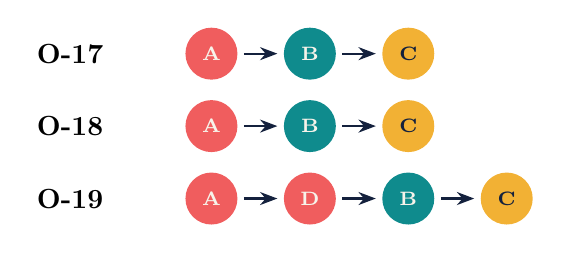
\begin{tikzpicture}[x=1.25cm,y=0.92cm]
    \node[anchor=east,font=\bfseries] at (0,2) {O-17};
    \node[event] at (1,2) {A}; \node[event,fill=Teal] at (2,2) {B};
    \node[event,fill=Gold,text=Ink] at (3,2) {C};
    \draw[flow] (1.33,2)--(1.67,2); \draw[flow] (2.33,2)--(2.67,2);

    \node[anchor=east,font=\bfseries] at (0,1) {O-18};
    \node[event] at (1,1) {A}; \node[event,fill=Teal] at (2,1) {B};
    \node[event,fill=Gold,text=Ink] at (3,1) {C};
    \draw[flow] (1.33,1)--(1.67,1); \draw[flow] (2.33,1)--(2.67,1);

    \node[anchor=east,font=\bfseries] at (0,0) {O-19};
    \node[event] at (1,0) {A}; \node[event,fill=Coral] at (2,0) {D};
    \node[event,fill=Teal] at (3,0) {B}; \node[event,fill=Gold,text=Ink] at (4,0) {C};
    \draw[flow] (1.33,0)--(1.67,0); \draw[flow] (2.33,0)--(2.67,0);
    \draw[flow] (3.33,0)--(3.67,0);
  \end{tikzpicture}

  \vspace{0.35cm}
  \begin{columns}[T,onlytextwidth]
    \column{0.46\textwidth}
      \textbf{Trace}: the ordered activity sequence for one case.
    \column{0.46\textwidth}
      \textbf{Variant}: a distinct trace pattern shared by cases.
  \end{columns}
  \vspace{0.25cm}
  Here: 3 cases, 2 variants.
\end{frame}

\begin{frame}{Lifecycle semantics change the answer}
  \begin{columns}[T,onlytextwidth]
    \column{0.55\textwidth}
      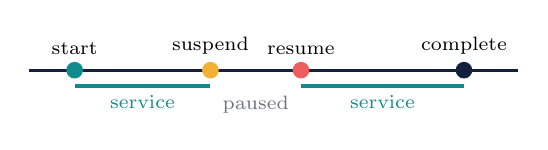
\begin{tikzpicture}[x=1.15cm,y=1cm]
        \draw[very thick,Ink] (0,0)--(5.4,0);
        \foreach \x/\lab/\col in {
          0.5/start/Teal,2.0/suspend/Gold,3.0/resume/Coral,4.8/complete/Ink}
          {
            \fill[\col] (\x,0) circle (3pt);
            \node[above,font=\scriptsize] at (\x,0.08) {\lab};
          }
        \draw[very thick,Teal] (0.5,-0.20)--(2.0,-0.20);
        \draw[very thick,Teal] (3.0,-0.20)--(4.8,-0.20);
        \node[below,font=\scriptsize,text=Teal] at (1.25,-0.2) {service};
        \node[below,font=\scriptsize,text=SoftGray] at (2.5,-0.2) {paused};
        \node[below,font=\scriptsize,text=Teal] at (3.9,-0.2) {service};
      \end{tikzpicture}
    \column{0.40\textwidth}
      \textbf{One activity may emit several events}
      \begin{itemize}
        \item Start
        \item Suspend / resume
        \item Complete
      \end{itemize}
  \end{columns}
  \vspace{0.45cm}
  \keyidea{Without lifecycle information, elapsed time may be mistaken for
  active work time.}
\end{frame}

\begin{frame}[fragile]{A first PM4Py event log}
\begin{lstlisting}[style=python]
import pandas as pd
import pm4py

events = pd.read_csv("orders.csv")
events["timestamp"] = pd.to_datetime(
    events["timestamp"], utc=True
)

events = pm4py.format_dataframe(
    events,
    case_id="case_id",
    activity_key="activity",
    timestamp_key="timestamp",
)

pm4py.write_xes(events, "orders.xes")
\end{lstlisting}
  \vspace{0.15cm}
  \textbf{Before running discovery:} verify identifiers, timestamps, ordering,
  duplicates, and event meaning.
\end{frame}

% ===========================================================================
% Unit 3
% ===========================================================================
\lecture{Event-Log Engineering and Data Quality}{03}
\section{Event-log engineering}
\unitdivider{03}{Event-Log Engineering and Data Quality}
  {An event log is a designed analytical artifact, not a raw database export.}

\begin{frame}{From source systems to an event log}
  \centering
  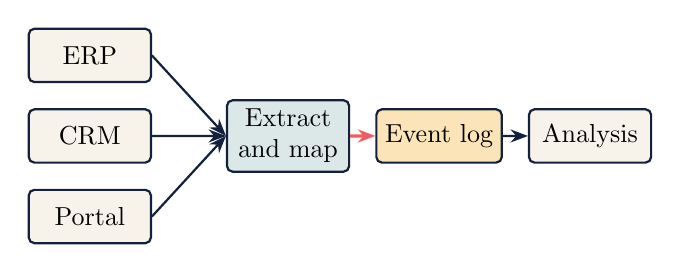
\begin{tikzpicture}[node distance=0.34cm,scale=0.94,transform shape]
    \node[activity] (erp) {ERP};
    \node[activity,below=of erp] (crm) {CRM};
    \node[activity,below=of crm] (web) {Portal};
    \node[activity,right=1.0cm of crm,fill=Mist] (etl) {Extract\\and map};
    \node[activity,right=of etl,fill=Gold!35] (log) {Event log};
    \node[activity,right=of log] (analysis) {Analysis};
    \draw[flow] (erp.east)--(etl.west);
    \draw[flow] (crm.east)--(etl.west);
    \draw[flow] (web.east)--(etl.west);
    \draw[accentflow] (etl)--(log);
    \draw[flow] (log)--(analysis);
  \end{tikzpicture}

  \vspace{0.55cm}
  Mapping decisions include:
  \begin{itemize}
    \item Which database change counts as a business event?
    \item How are records correlated into cases?
    \item Which timestamps and time zones are authoritative?
    \item Which low-level events should be abstracted?
  \end{itemize}
\end{frame}

\begin{frame}{Six common data-quality traps}
  \begin{columns}[T,onlytextwidth]
    \column{0.47\textwidth}
      \begin{enumerate}
        \item Missing events
        \item Duplicate events
        \item Incorrect ordering
      \end{enumerate}
    \column{0.47\textwidth}
      \begin{enumerate}
        \setcounter{enumi}{3}
        \item Mixed granularity
        \item Unstable case identifiers
        \item Selection and extraction bias
      \end{enumerate}
  \end{columns}
  \vspace{0.55cm}
  \begin{block}{Diagnostic habit}
    For every surprising pattern, ask: \textit{Is this process behavior,
    logging behavior, or extraction behavior?}
  \end{block}
\end{frame}

\begin{frame}{The case-notion test}
  A useful case notion should satisfy three questions:
  \begin{enumerate}
    \item Do the grouped events belong to the same process instance?
    \item Does the resulting sequence have a meaningful beginning and end?
    \item Does it support the decision the analysis is meant to inform?
  \end{enumerate}
  \vspace{0.4cm}
  \begin{columns}[T,onlytextwidth]
    \column{0.46\textwidth}
      \begin{block}{Order as case}
        Good for customer lead time and order completion.
      \end{block}
    \column{0.46\textwidth}
      \begin{block}{Item as case}
        Better for partial fulfillment and item-level handling.
      \end{block}
  \end{columns}
\end{frame}

\begin{frame}{A compact quality report}
  \small
  \begin{tabular}{@{}p{0.26\textwidth}p{0.26\textwidth}p{0.36\textwidth}@{}}
    \toprule
    Check & Evidence & Decision / limitation\\
    \midrule
    Case completeness & 8.4\% lack an end event & Exclude open cases from cycle-time KPI\\
    Timestamp order & 23 negative intervals & Correct known clock offset; flag remainder\\
    Duplicates & 1.2\% exact duplicates & Remove with documented key\\
    Activity meaning & ``Update'' has 4 sources & Split by business semantics\\
    Coverage & Data begins Jan 2025 & No claims about earlier process versions\\
    \bottomrule
  \end{tabular}
  \vspace{0.45cm}
  \keyidea{Documenting exclusions is part of the result, not administrative
  overhead.}
\end{frame}

\begin{frame}{Profile before you transform}
  \small
  \begin{tabular}{@{}p{0.19\textwidth}p{0.28\textwidth}p{0.42\textwidth}@{}}
    \toprule
    Level & Profile & Decision it informs\\
    \midrule
    Event & Missingness, duplicates, timestamps & Repair, exclude, or reinterpret\\
    Case & Length, duration, completeness & Boundaries and open-case policy\\
    Activity & Frequency, lifecycle, resources & Abstraction and filtering\\
    Variant & Coverage, rarity, entropy & Noise strategy and segmentation\\
    Temporal & Volume, drift, seasonality & Time windows and evaluation split\\
    \bottomrule
  \end{tabular}
  \vspace{0.45cm}
  \keyidea{Profiling is not merely descriptive. It determines which
  transformations, models, and evaluation designs are defensible.}
\end{frame}

\begin{frame}{Flattening is a modeling choice}
  \begin{columns}[T,onlytextwidth]
    \column{0.54\textwidth}
      \centering
      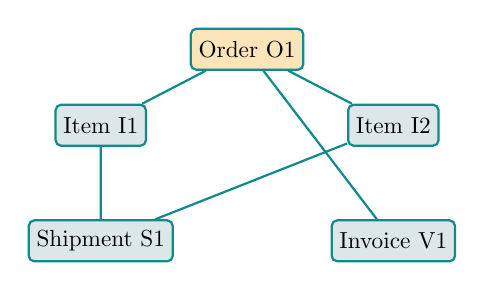
\begin{tikzpicture}[node distance=0.5cm and 0.65cm,scale=0.84,transform shape]
        \node[object,fill=Gold!35] (order) {Order O1};
        \node[object,below left=of order] (i1) {Item I1};
        \node[object,below right=of order] (i2) {Item I2};
        \node[object,below=1.1cm of i1] (ship) {Shipment S1};
        \node[object,below=1.1cm of i2] (inv) {Invoice V1};
        \draw[Teal,thick] (order)--(i1);
        \draw[Teal,thick] (order)--(i2);
        \draw[Teal,thick] (i1)--(ship);
        \draw[Teal,thick] (i2)--(ship);
        \draw[Teal,thick] (order)--(inv);
      \end{tikzpicture}
    \column{0.41\textwidth}
      \textbf{Flatten by order}
      \begin{itemize}
        \item Shared item events converge
      \end{itemize}
      \textbf{Flatten by item}
      \begin{itemize}
        \item Shared order events duplicate
      \end{itemize}
      \textbf{Keep objects}
      \begin{itemize}
        \item Relationships remain explicit
      \end{itemize}
  \end{columns}
  \vspace{0.35cm}
  \promptbox{Which case notion preserves the behavior needed by your question,
  and which frequencies does it distort?}
\end{frame}

\begin{frame}{Flattening and encoding: two layers, two decisions}
  \centering
  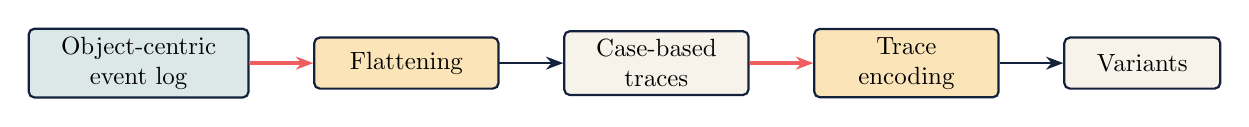
\begin{tikzpicture}[node distance=0.5cm and 0.9cm,scale=0.9,transform shape]
    \node[activity,fill=Mist,minimum width=3.1cm] (raw) {Object-centric\\event log};
    \node[activity,right=of raw,fill=Gold!35,minimum width=2.6cm] (flat) {Flattening};
    \node[activity,right=of flat,minimum width=2.6cm] (cases) {Case-based\\traces};
    \node[activity,right=of cases,fill=Gold!35,minimum width=2.6cm] (enc) {Trace\\encoding};
    \node[activity,right=of enc,minimum width=2.2cm] (var) {Variants};
    \draw[accentflow] (raw)--(flat);
    \draw[flow] (flat)--(cases);
    \draw[accentflow] (cases)--(enc);
    \draw[flow] (enc)--(var);
  \end{tikzpicture}
  \vspace{0.45cm}
  \begin{columns}[T,onlytextwidth]
    \column{0.47\textwidth}
      \begin{block}{Flattening}
        Decides \textbf{which events belong to the same case}. Coarser,
        earlier: it chooses the case notion (order, item, shipment\ldots)
        and creates convergence or divergence before any trace exists.
      \end{block}
    \column{0.47\textwidth}
      \begin{block}{Encoding}
        Decides \textbf{how an already-defined case is represented} as a
        trace: control-flow, lifecycle, time, or payload. Finer, later: it
        shapes variants once cases already exist.
      \end{block}
  \end{columns}
  \vspace{0.3cm}
  \keyidea{Both are modeling choices, not neutral defaults: flattening
  fixes what counts as one case, encoding fixes how that case's history is
  read.}
\end{frame}

% ===========================================================================
% Unit 4
% ===========================================================================
\lecture{Exploratory Process Analysis}{04}
\section{Exploratory analysis}
\unitdivider{04}{Exploratory Process Analysis}
  {Build a map of the evidence before building a process model.}

\begin{frame}{Explore at four levels}
  \begin{columns}[T,onlytextwidth]
    \column{0.22\textwidth}
      \begin{block}{Log}
        Cases, events, date range, coverage
      \end{block}
    \column{0.22\textwidth}
      \begin{block}{Case}
        Duration, event count, outcomes
      \end{block}
    \column{0.22\textwidth}
      \begin{block}{Activity}
        Frequency, resources, timing
      \end{block}
    \column{0.22\textwidth}
      \begin{block}{Variant}
        Paths, prevalence, performance
      \end{block}
  \end{columns}
  \vspace{0.55cm}
  \promptbox{Which level would reveal rework? Which would reveal a seasonal
  extraction gap?}
\end{frame}

\begin{frame}{A directly-follows graph}
  \centering
  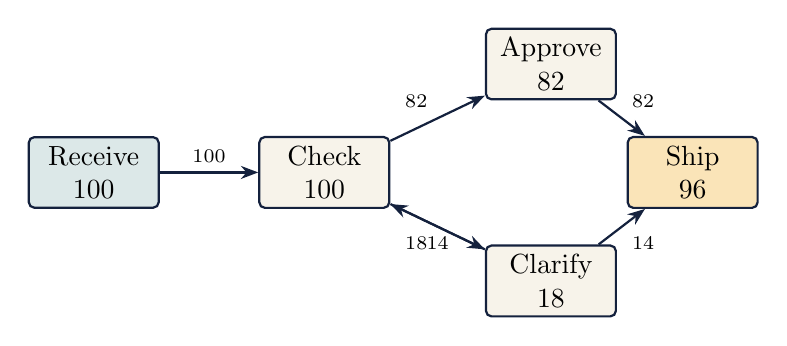
\begin{tikzpicture}[node distance=1.0cm and 1.25cm]
    \node[activity,fill=Mist] (a) {Receive\\100};
    \node[activity,right=of a] (b) {Check\\100};
    \node[activity,above right=0.45cm and 1.2cm of b] (c) {Approve\\82};
    \node[activity,below right=0.45cm and 1.2cm of b] (d) {Clarify\\18};
    \node[activity,right=3.0cm of b,fill=Gold!35] (e) {Ship\\96};
    \draw[flow] (a)--node[above,font=\scriptsize]{100}(b);
    \draw[flow] (b)--node[above left,font=\scriptsize]{82}(c);
    \draw[flow] (b)--node[below left,font=\scriptsize]{18}(d);
    \draw[flow] (d)--node[below,font=\scriptsize]{14}(b);
    \draw[flow] (c)--node[above right,font=\scriptsize]{82}(e);
    \draw[flow] (d)--node[below right,font=\scriptsize]{14}(e);
  \end{tikzpicture}

  \vspace{0.45cm}
  A DFG summarizes observed adjacency:
  \begin{itemize}
    \item Nodes are activities; edges mean ``directly followed by''
    \item Counts can represent frequency or performance
    \item Loops, choices, and concurrency require careful interpretation
  \end{itemize}
\end{frame}

\begin{frame}{Variants: useful, but easy to misuse}
  \small
  \begin{tabular}{@{}clrr@{}}
    \toprule
    Rank & Variant & Cases & Median time\\
    \midrule
    1 & Receive, Check, Approve, Ship & 68\% & 2.1 d\\
    2 & Receive, Check, Clarify, Check, Ship & 14\% & 5.8 d\\
    3 & Receive, Check, Reject & 8\% & 1.4 d\\
    4+ & 17 other variants & 10\% & 8.2 d\\
    \bottomrule
  \end{tabular}
  \vspace{0.45cm}
  \begin{columns}[T,onlytextwidth]
    \column{0.47\textwidth}
      \textbf{Variants reveal}
      \begin{itemize}
        \item Dominant routes
        \item Rework patterns
        \item Exceptional behavior
      \end{itemize}
    \column{0.47\textwidth}
      \textbf{Variants can hide}
      \begin{itemize}
        \item Concurrent behavior
        \item Attribute differences
        \item Important rare cases
      \end{itemize}
  \end{columns}
\end{frame}

\begin{frame}{A variant depends on its trace encoding}
  \small
  \begin{tabular}{@{}
    >{\raggedright\arraybackslash}p{0.24\textwidth}
    >{\raggedright\arraybackslash}p{0.36\textwidth}
    >{\raggedright\arraybackslash}p{0.31\textwidth}@{}}
    \toprule
    Encoding & Trace representation & Variants distinguish\\
    \midrule
    Control-flow & Activity sequence & Routing differences\\
    Lifecycle-aware & Activity + transition & Start, suspend, resume, complete\\
    Time-aware & Activity + duration bucket & Behavioral and timing regimes\\
    Payload-aware & Activity + selected attributes & Context or outcome cohorts\\
    Learned & Sequence / payload embedding & Similarity beyond exact equality\\
    \bottomrule
  \end{tabular}
  \vspace{0.4cm}
  \keyidea{Variant counts are not properties of the raw log alone. They are
  produced by an encoding, equivalence rule, and similarity threshold.}
\end{frame}

\begin{frame}{Profile the payload before using it}
  \small
  \begin{columns}[T,onlytextwidth]
    \column{0.46\textwidth}
      \begin{block}{Event payload}
        Information carried by an event beyond case, activity, and timestamp.
      \end{block}
      \begin{itemize}
        \item Structured attributes and measurements
        \item Text, documents, images, audio, and sensor references
        \item Resource, cost, location, and product context
      \end{itemize}
    \column{0.46\textwidth}
      \textbf{Profile before encoding}
      \begin{itemize}
        \item Availability at event time
        \item Missingness and cardinality
        \item Drift, semantics, and cardinality
        \item Privacy, proxies, and future leakage
      \end{itemize}
  \end{columns}
  \vspace{0.05cm}
  \promptbox{Use payload dimensions only when they serve the analytical question;
  otherwise they can fragment traces into meaningless one-case variants.}
\end{frame}

\begin{frame}{Pareto front for trace-variant detection}
  \scriptsize
  \begin{columns}[T,onlytextwidth]
    \column{0.56\textwidth}
      \centering
      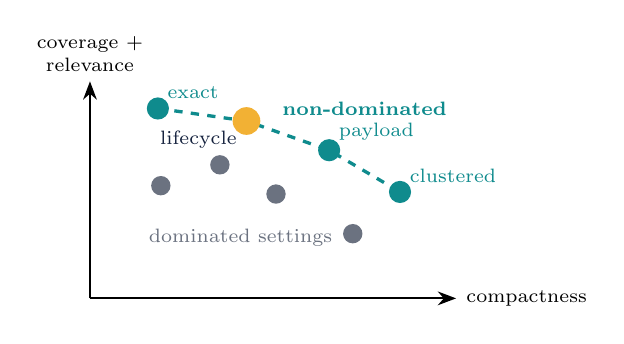
\begin{tikzpicture}[x=0.75cm,y=0.53cm]
        \draw[-{Stealth},thick] (0,0)--(6.2,0)
          node[right,font=\scriptsize]{compactness};
        \draw[-{Stealth},thick] (0,0)--(0,5.2)
          node[above,font=\scriptsize,align=center]{coverage +\\relevance};

        \draw[Teal,very thick,dashed]
          (1.15,4.55)--(2.65,4.25)--(4.05,3.55)--(5.25,2.55);
        \fill[Teal] (1.15,4.55) circle (4pt)
          node[above right,font=\scriptsize]{exact};
        \fill[Gold] (2.65,4.25) circle (5pt)
          node[below left,font=\scriptsize,text=Ink]{lifecycle};
        \fill[Teal] (4.05,3.55) circle (4pt)
          node[above right,font=\scriptsize]{payload};
        \fill[Teal] (5.25,2.55) circle (4pt)
          node[above right,font=\scriptsize]{clustered};

        \foreach \x/\y in {1.2/2.7,2.2/3.2,3.15/2.5,4.45/1.55}
          \fill[SoftGray] (\x,\y) circle (3.5pt);
        \node[Teal,font=\scriptsize\bfseries] at (4.65,4.55)
          {non-dominated};
        \node[SoftGray,font=\scriptsize] at (2.55,1.45)
          {dominated settings};
      \end{tikzpicture}
    \column{0.39\textwidth}
      \textbf{Candidate settings}\\
      Encoding, similarity threshold, rare-variant cutoff, and payload dimensions.

      \vspace{0.25cm}
      \textbf{Objectives}\\
      Case coverage, compactness, decision relevance, and temporal stability.
  \end{columns}
  \vspace{0.1cm}
  \centering\textbf{\color{Teal}Inspect representative traces before selecting
  a non-dominated setting.}
\end{frame}

\begin{frame}{A modeling-readiness profile}
  Before discovery or prediction, record:
  \begin{columns}[T,onlytextwidth]
    \column{0.47\textwidth}
      \begin{itemize}
        \item Case and trace-length distributions
        \item Variant coverage and long-tail behavior
        \item Class and outcome imbalance
        \item Missing and high-cardinality attributes
      \end{itemize}
    \column{0.47\textwidth}
      \begin{itemize}
        \item Process and population drift
        \item Open versus completed cases
        \item Observation and label timestamps
        \item Potential future-information leakage
      \end{itemize}
  \end{columns}
  \vspace{0.4cm}
  \begin{block}{Deliverable}
    A one-page readiness report: usable population, known distortions,
    representation choice, split strategy, and excluded information.
  \end{block}
\end{frame}

\begin{frame}[fragile]{PM4Py exploration}
\begin{lstlisting}[style=python]
import pm4py

print(pm4py.get_start_activities(log))
print(pm4py.get_end_activities(log))

variants = pm4py.get_variants_as_tuples(log)
dfg, starts, ends = pm4py.discover_dfg(log)

filtered = pm4py.filter_case_performance(
    log,
    min_performance=5 * 24 * 60 * 60,
)
\end{lstlisting}
  \vspace{0.15cm}
  \textbf{Interpretation task:} compare common cases with slow cases. Which
  path differences are plausible explanations, and which need more evidence?
\end{frame}

% ===========================================================================
% Unit 5
% ===========================================================================
\lecture{Process-Modeling Foundations}{05}
\section{Modeling foundations}
\unitdivider{05}{Process-Modeling Foundations}
  {Different representations answer different questions.}

\begin{frame}{Four behavioral building blocks}
  \begin{columns}[T,onlytextwidth]
    \column{0.22\textwidth}
      \begin{block}{Sequence}
        $A \rightarrow B$
      \end{block}
      One follows another.
    \column{0.22\textwidth}
      \begin{block}{Choice}
        $A \rightarrow (B|C)$
      \end{block}
      One branch is selected.
    \column{0.22\textwidth}
      \begin{block}{Parallel}
        $A \rightarrow (B \parallel C)$
      \end{block}
      Both occur, order varies.
    \column{0.22\textwidth}
      \begin{block}{Loop}
        $A \rightarrow B \rightarrow A$
      \end{block}
      Behavior repeats.
  \end{columns}
  \vspace{0.55cm}
  \keyidea{A useful model must distinguish choice from concurrency and permit
  repetition without permitting everything.}
\end{frame}

\begin{frame}{A DFG is not a complete process model}
  \begin{columns}[T,onlytextwidth]
    \column{0.48\textwidth}
      \centering
      \textbf{Observed traces}\\[0.25cm]
      $\langle A,B,C,D\rangle$\\
      $\langle A,C,B,D\rangle$\\[0.45cm]
      Evidence suggests $B$ and $C$ may be parallel.
    \column{0.48\textwidth}
      \centering
      \textbf{DFG}\\[0.2cm]
      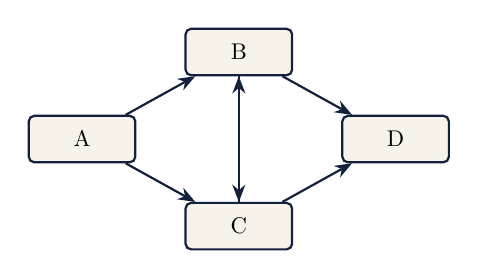
\begin{tikzpicture}[node distance=0.6cm and 0.75cm,scale=0.82,transform shape]
        \node[activity] (a) {A};
        \node[activity,above right=of a] (b) {B};
        \node[activity,below right=of a] (c) {C};
        \node[activity,below right=of b] (d) {D};
        \draw[flow] (a)--(b); \draw[flow] (a)--(c);
        \draw[flow] (b)--(c); \draw[flow] (c)--(b);
        \draw[flow] (b)--(d); \draw[flow] (c)--(d);
      \end{tikzpicture}
  \end{columns}
  \vspace{0.55cm}
  The DFG also appears to allow repeated alternation between $B$ and $C$.
  That behavior was never observed.
\end{frame}

\begin{frame}[shrink=8]{Model representations}
  \centering
  \begin{columns}[T,onlytextwidth]
    \column{0.24\textwidth}
      \centering
      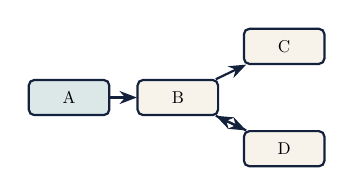
\begin{tikzpicture}[scale=0.62,transform shape,node distance=0.4cm and 0.55cm]
        \node[activity,fill=Mist] (a) {A};
        \node[activity,right=of a] (b) {B};
        \node[activity,above right=0.3cm and 0.5cm of b] (c) {C};
        \node[activity,below right=0.3cm and 0.5cm of b] (d) {D};
        \draw[flow] (a)--(b);
        \draw[flow] (b)--(c);
        \draw[flow] (b)--(d);
        \draw[flow] (d)--(b);
      \end{tikzpicture}
      \textbf{DFG}\\[0.15cm]
      \textit{Strength:} fast, readable overview\\
      \textit{Watch for:} no complete execution semantics
    \column{0.24\textwidth}
      \centering
      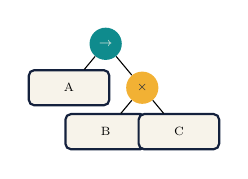
\begin{tikzpicture}[scale=0.62,transform shape,
          level distance=0.9cm,sibling distance=1.5cm,
          every node/.style={font=\scriptsize}]
        \node[event,fill=Teal] {$\rightarrow$}
          child { node[activity] {A} }
          child { node[event,fill=Gold,text=Ink] {$\times$}
            child { node[activity] {B} }
            child { node[activity] {C} }
          };
      \end{tikzpicture}
      \textbf{Process tree}\\[0.15cm]
      \textit{Strength:} structured, sound by construction\\
      \textit{Watch for:} restricts model shape
    \column{0.24\textwidth}
      \centering
      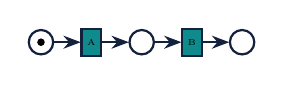
\begin{tikzpicture}[scale=0.62,transform shape,
          place/.style={circle,draw=Ink,thick,minimum size=0.5cm},
          trans/.style={rectangle,draw=Ink,thick,fill=Teal,
            minimum width=0.4cm,minimum height=0.55cm},
          node distance=0.55cm]
        \node[place] (p0) {};
        \fill (p0) circle (2.2pt);
        \node[trans,right=of p0] (t1) {\tiny A};
        \node[place,right=of t1] (p1) {};
        \node[trans,right=of p1] (t2) {\tiny B};
        \node[place,right=of t2] (p2) {};
        \draw[flow] (p0)--(t1); \draw[flow] (t1)--(p1);
        \draw[flow] (p1)--(t2); \draw[flow] (t2)--(p2);
      \end{tikzpicture}
      \textbf{Petri net}\\[0.15cm]
      \textit{Strength:} precise concurrency and replay\\
      \textit{Watch for:} harder for non-specialists
    \column{0.24\textwidth}
      \centering
      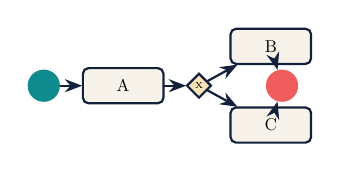
\begin{tikzpicture}[scale=0.62,transform shape,node distance=0.45cm]
        \node[event,fill=Teal] (s) {};
        \node[activity,right=of s] (a) {A};
        \node[shape=diamond,draw=Ink,thick,fill=Gold!35,
          minimum size=0.5cm,right=of a,inner sep=0pt] (g) {\tiny X};
        \node[activity,above right=0.3cm and 0.5cm of g] (b) {B};
        \node[activity,below right=0.3cm and 0.5cm of g] (c) {C};
        \node[event,fill=Coral,right=1.1cm of g] (e) {};
        \draw[flow] (s)--(a); \draw[flow] (a)--(g);
        \draw[flow] (g)--(b); \draw[flow] (g)--(c);
        \draw[flow] (b)--(e); \draw[flow] (c)--(e);
      \end{tikzpicture}
      \textbf{BPMN}\\[0.15cm]
      \textit{Strength:} familiar business notation\\
      \textit{Watch for:} semantics vary by usage
  \end{columns}
  \vspace{0.4cm}
  \promptbox{Which representation would you use for stakeholder discussion?
  Which for alignment-based conformance checking?}
\end{frame}

\begin{frame}{Choose a modeling strategy}
  \small
  \begin{tabular}{@{}
    >{\raggedright\arraybackslash}p{0.19\textwidth}
    >{\raggedright\arraybackslash}p{0.23\textwidth}
    >{\raggedright\arraybackslash}p{0.24\textwidth}
    >{\raggedright\arraybackslash}p{0.24\textwidth}@{}}
    \toprule
    Purpose & Strategy & Representation & Emphasize\\
    \midrule
    Explain flow & Structured discovery & Process tree / BPMN & Simplicity, fitness\\
    Audit rules & Normative modeling & Petri net / Declare & Soundness, diagnostics\\
    Explore complexity & Frequency-aware discovery & DFG / heuristics net & Coverage, readability\\
    Predict state & State or prefix model & Transition / features & Generalization, utility\\
    Communicate & Simplify and annotate & BPMN / DFG & Interpretability\\
    \bottomrule
  \end{tabular}
  \vspace{0.45cm}
  \keyidea{There is no context-free ``best model.'' State the purpose before
  selecting the algorithm, representation, and quality criteria.}
\end{frame}

\begin{frame}{Abstraction before algorithm}
  \centering
  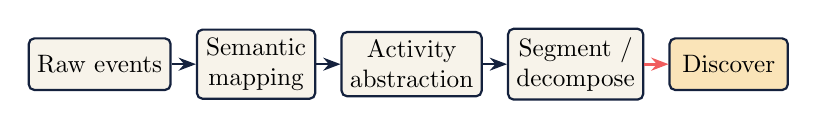
\begin{tikzpicture}[node distance=0.34cm,scale=0.91,transform shape]
    \node[activity] (raw) {Raw events};
    \node[activity,right=of raw] (semantic) {Semantic\\mapping};
    \node[activity,right=of semantic] (abstract) {Activity\\abstraction};
    \node[activity,right=of abstract] (segment) {Segment /\\decompose};
    \node[activity,right=of segment,fill=Gold!35] (discover) {Discover};
    \draw[flow] (raw)--(semantic);
    \draw[flow] (semantic)--(abstract);
    \draw[flow] (abstract)--(segment);
    \draw[accentflow] (segment)--(discover);
  \end{tikzpicture}
  \vspace{0.55cm}
  \begin{columns}[T,onlytextwidth]
    \column{0.47\textwidth}
      \textbf{Useful strategies}
      \begin{itemize}
        \item Collapse technical events
        \item Separate process populations
        \item Decompose by lifecycle or subprocess
      \end{itemize}
    \column{0.47\textwidth}
      \textbf{Practice}
      \begin{itemize}
        \item Version every mapping
        \item Compare before and after profiles
        \item Retain a traceable raw-event link
      \end{itemize}
  \end{columns}
\end{frame}

\begin{frame}{Soundness: can every case finish properly?}
  For a workflow model, we usually want:
  \begin{itemize}
    \item One meaningful start and one meaningful completion
    \item Every modeled activity can occur
    \item No deadlocks before completion
    \item No tokens or work left behind after completion
  \end{itemize}
  \vspace{0.35cm}
  \begin{block}{Why it matters}
    An attractive diagram can still encode impossible or incomplete behavior.
    Formal semantics let us test the model rather than trust its appearance.
  \end{block}
\end{frame}

% ===========================================================================
% Unit 6
% ===========================================================================
\lecture{Process Discovery}{06}
\section{Process discovery}
\unitdivider{06}{Process Discovery}
  {Discovery algorithms compress event behavior into an explanatory model.}

\begin{frame}{Discovery is a balancing act}
  \centering
  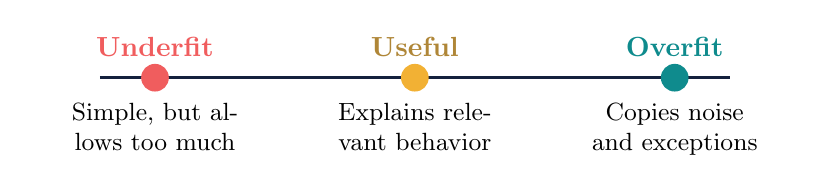
\begin{tikzpicture}
    \draw[very thick,Ink] (-4,0)--(4,0);
    \fill[Coral] (-3.3,0) circle (5pt);
    \fill[Gold] (0,0) circle (5pt);
    \fill[Teal] (3.3,0) circle (5pt);
    \node[above,text=Coral,font=\bfseries] at (-3.3,0.15) {Underfit};
    \node[above,text=Gold!70!Ink,font=\bfseries] at (0,0.15) {Useful};
    \node[above,text=Teal,font=\bfseries] at (3.3,0.15) {Overfit};
    \node[below,text width=3cm,align=center,font=\small] at (-3.3,-0.2)
      {Simple, but allows too much};
    \node[below,text width=3cm,align=center,font=\small] at (0,-0.2)
      {Explains relevant behavior};
    \node[below,text width=3cm,align=center,font=\small] at (3.3,-0.2)
      {Copies noise and exceptions};
  \end{tikzpicture}
  \vspace{0.8cm}
  Discovery depends on:
  \begin{itemize}
    \item The event log and its abstraction level
    \item The algorithm's behavioral assumptions
    \item Noise and frequency thresholds
    \item The intended use of the resulting model
  \end{itemize}
\end{frame}

\begin{frame}{Three discovery families}
  \begin{columns}[T,onlytextwidth]
    \column{0.30\textwidth}
      \begin{block}{Alpha Miner}
        Uses ordering relations to infer causal, parallel, and choice behavior.
      \end{block}
      Best as a conceptual foundation.
    \column{0.30\textwidth}
      \begin{block}{Heuristics Miner}
        Uses frequency and dependency measures to tolerate noise.
      \end{block}
      Useful for exploratory models.
    \column{0.30\textwidth}
      \begin{block}{Inductive Miner}
        Recursively finds sequence, choice, parallel, and loop cuts.
      \end{block}
      Produces sound, structured models.
  \end{columns}
\end{frame}

\begin{frame}{A disciplined discovery experiment}
  \centering
  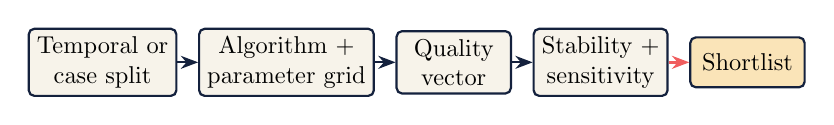
\begin{tikzpicture}[node distance=0.30cm,scale=0.88,transform shape]
    \node[activity] (split) {Temporal or\\case split};
    \node[activity,right=of split] (grid) {Algorithm +\\parameter grid};
    \node[activity,right=of grid] (quality) {Quality\\vector};
    \node[activity,right=of quality] (stable) {Stability +\\sensitivity};
    \node[activity,right=of stable,fill=Gold!35] (short) {Shortlist};
    \draw[flow] (split)--(grid);
    \draw[flow] (grid)--(quality);
    \draw[flow] (quality)--(stable);
    \draw[accentflow] (stable)--(short);
  \end{tikzpicture}
  \vspace{0.55cm}
  \begin{enumerate}
    \item Define constraints and metric directions before seeing results.
    \item Keep discovery data separate from final evaluation data.
    \item Retain all candidate parameters and artifacts, not only the winner.
    \item Inspect unstable activities and edges, not only aggregate scores.
  \end{enumerate}
\end{frame}

\begin{frame}{Inductive discovery intuition}
  \centering
  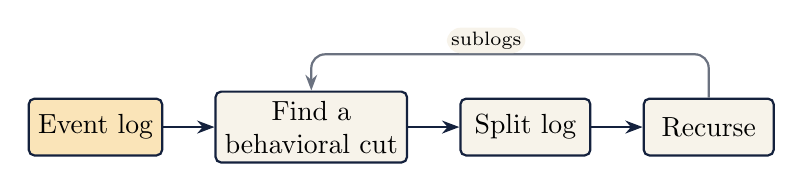
\begin{tikzpicture}[node distance=0.45cm and 0.65cm]
    \node[activity,fill=Gold!35] (log) {Event log};
    \node[activity,right=of log] (cut) {Find a\\behavioral cut};
    \node[activity,right=of cut] (split) {Split log};
    \node[activity,right=of split] (rec) {Recurse};
    \draw[flow] (log)--(cut);
    \draw[flow] (cut)--(split);
    \draw[flow] (split)--(rec);
    \draw[softflow,rounded corners=5pt]
      (rec.north) -- ++(0,0.55)
      -| node[pos=0.28,above,font=\scriptsize,fill=Paper,inner sep=1.5pt]
        {sublogs}
      (cut.north);
  \end{tikzpicture}
  \vspace{0.55cm}
  Candidate cuts:
  \begin{columns}[T,onlytextwidth]
    \column{0.22\textwidth}\centering Sequence\\$\rightarrow$
    \column{0.22\textwidth}\centering Exclusive choice\\$\times$
    \column{0.22\textwidth}\centering Parallel\\$\wedge$
    \column{0.22\textwidth}\centering Loop\\$\circlearrowleft$
  \end{columns}
  \vspace{0.45cm}
  \keyidea{The result is a process tree that can be translated into a Petri net
  or BPMN model.}
\end{frame}

\begin{frame}[fragile]{Discover with PM4Py}
\begin{lstlisting}[style=python]
import pm4py

# Structured discovery
tree = pm4py.discover_process_tree_inductive(
    log, noise_threshold=0.2
)
net, initial, final = pm4py.convert_to_petri_net(tree)

# Business-facing representation
bpmn = pm4py.convert_to_bpmn(tree)
pm4py.save_vis_bpmn(bpmn, "discovered_process.svg")
\end{lstlisting}
  \vspace{0.15cm}
  \textbf{Experiment:} vary the noise threshold. Record which behavior disappears,
  which remains, and whether the model becomes more useful.
\end{frame}

% ===========================================================================
% Unit 7
% ===========================================================================
\lecture{Model Quality and Evaluation}{07}
\section{Model quality}
\unitdivider{07}{Model Quality and Evaluation}
  {No single score can tell you whether a model is fit for purpose.}

\begin{frame}{The four quality dimensions}
  \begin{columns}[T,onlytextwidth]
    \column{0.22\textwidth}
      \begin{block}{Fitness}
        Can the model replay observed behavior?
      \end{block}
    \column{0.22\textwidth}
      \begin{block}{Precision}
        Does it avoid allowing unseen behavior?
      \end{block}
    \column{0.22\textwidth}
      \begin{block}{Generalization}
        Does it handle plausible future behavior?
      \end{block}
    \column{0.22\textwidth}
      \begin{block}{Simplicity}
        Can people understand and use it?
      \end{block}
  \end{columns}
  \vspace{0.55cm}
  \keyidea{Perfect fitness is trivial if the model allows every possible trace.
  Quality emerges from the trade-off.}
\end{frame}

\begin{frame}{Build a quality vector, not one score}
  \scriptsize
  \begin{tabular}{@{}p{0.20\textwidth}p{0.32\textwidth}p{0.36\textwidth}@{}}
    \toprule
    Dimension & Example measure & Interpretation risk\\
    \midrule
    Fitness & Alignment / replay fitness & Rewards permissive models\\
    Precision & Escaping-edge / alignment precision & Sensitive to log coverage\\
    Generalization & Holdout replay, cross-validation & Depends on split design\\
    Simplicity & Nodes, arcs, control-flow complexity & Small is not always understandable\\
    Stability & Bootstrap edge / relation frequency & Aggregate scores can hide churn\\
    Feasibility & Soundness, runtime, memory & Hard constraints, not preferences\\
    \bottomrule
  \end{tabular}
  \vspace{0.2cm}
  \keyidea{Record metric direction, computation method, dataset split, and
  uncertainty for every component of the quality vector.}
\end{frame}

\begin{frame}{Fitness and precision pull in opposite directions}
  \centering
  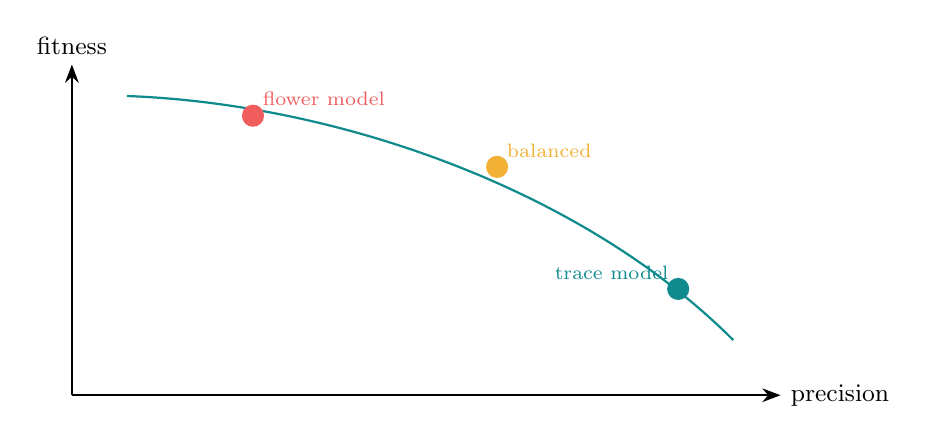
\begin{tikzpicture}[x=1cm,y=1cm]
    \draw[-{Stealth},thick] (0,0)--(9,0) node[right,font=\small]{precision};
    \draw[-{Stealth},thick] (0,0)--(0,4.2) node[above,font=\small]{fitness};
    \draw[thick,Teal] (0.7,3.8) .. controls (3.4,3.7) and (6.5,2.6) .. (8.4,0.7);
    \fill[Coral] (2.3,3.55) circle (4pt) node[above right,font=\scriptsize]{flower model};
    \fill[Gold] (5.4,2.9) circle (4pt) node[above right,font=\scriptsize]{balanced};
    \fill[Teal] (7.7,1.35) circle (4pt) node[above left,font=\scriptsize]{trace model};
  \end{tikzpicture}
  \par
  \vspace{0.25cm}
  The ``best'' point depends on whether the model is for explanation,
  simulation, compliance, or prediction.
\end{frame}

\begin{frame}{Why a weighted average can mislead}
  Suppose:
  \[
    score = 0.4\,fitness + 0.4\,precision + 0.2\,simplicity
  \]
  \begin{columns}[T,onlytextwidth]
    \column{0.47\textwidth}
      \textbf{What it hides}
      \begin{itemize}
        \item A critical minimum may be violated
        \item Different weights reverse the ranking
        \item Compensating metrics may be unacceptable
        \item Scale and normalization alter the result
      \end{itemize}
    \column{0.47\textwidth}
      \textbf{Better first step}
      \begin{itemize}
        \item Apply hard feasibility constraints
        \item Remove dominated candidates
        \item Inspect the Pareto front
        \item Add preferences only afterward
      \end{itemize}
  \end{columns}
\end{frame}

\begin{frame}{Pareto dominance and the Pareto front}
  \begin{columns}[T,onlytextwidth]
    \column{0.57\textwidth}
      \centering
      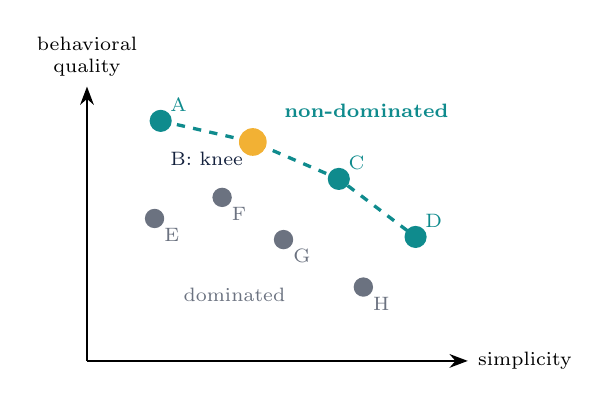
\begin{tikzpicture}[x=0.78cm,y=0.67cm]
        \draw[-{Stealth},thick] (0,0)--(6.2,0)
          node[right,font=\scriptsize]{simplicity};
        \draw[-{Stealth},thick] (0,0)--(0,5.2)
          node[above,font=\scriptsize,align=center]{behavioral\\quality};

        \draw[Teal,very thick,dashed]
          (1.2,4.55)--(2.7,4.15)--(4.1,3.45)--(5.35,2.35);
        \foreach \x/\y/\lab in {
          1.2/4.55/A,4.1/3.45/C,5.35/2.35/D}
          \fill[Teal] (\x,\y) circle (4pt)
            node[above right,font=\scriptsize]{\lab};
        \fill[Gold] (2.7,4.15) circle (5pt)
          node[below left,font=\scriptsize,text=Ink]{B: knee};

        \foreach \x/\y/\lab in {
          1.1/2.7/E,2.2/3.1/F,3.2/2.3/G,4.5/1.4/H}
          \fill[SoftGray] (\x,\y) circle (3.5pt)
            node[below right,font=\scriptsize]{\lab};
        \node[Teal,font=\scriptsize\bfseries] at (4.55,4.75)
          {non-dominated};
        \node[SoftGray,font=\scriptsize] at (2.4,1.25)
          {dominated};
      \end{tikzpicture}
    \column{0.38\textwidth}
      Candidate $X$ dominates $Y$ when:
      \begin{itemize}
        \item $X$ is no worse on every objective
        \item $X$ is better on at least one objective
      \end{itemize}
      \vspace{0.1cm}
      The \textbf{Pareto front} contains candidates not dominated by any other
      candidate.
  \end{columns}
  \vspace{0.05cm}
  \keyidea{A knee point offers a strong trade-off, but it is a candidate for
  discussion, not an automatic winner.}
\end{frame}

\begin{frame}{Practical Pareto-front selection}
  \begin{enumerate}
    \item \textbf{Constrain first}: require soundness, minimum fitness, and an
      acceptable runtime or model size.
    \item \textbf{Estimate uncertainty}: bootstrap cases or repeat temporal
      folds; do not trust tiny score differences.
    \item \textbf{Inspect sensitivity}: vary thresholds, activity abstraction,
      and metric implementation.
    \item \textbf{Review the front}: show all non-dominated models and explain
      what is gained and lost between adjacent candidates.
    \item \textbf{Select transparently}: use a knee point, lexicographic rule,
      or stakeholder utility after the front is known.
    \item \textbf{Validate once}: report the final choice on untouched holdout
      data.
  \end{enumerate}
\end{frame}

\begin{frame}{Replay and alignments}
  \begin{columns}[T,onlytextwidth]
    \column{0.47\textwidth}
      \begin{block}{Token-based replay}
        Replays traces on a Petri net and counts missing, remaining, consumed,
        and produced tokens.
      \end{block}
      Fast and diagnostic, but can mask some deviations.
    \column{0.47\textwidth}
      \begin{block}{Alignments}
        Find a minimum-cost correspondence between log behavior and model
        behavior.
      \end{block}
      More precise, but computationally more expensive.
  \end{columns}
  \vspace{0.55cm}
  \promptbox{Would you evaluate a compliance model and an exploratory model with
  the same tolerance for deviations? Why?}
\end{frame}

\begin{frame}[fragile]{Evaluate candidates}
\begin{lstlisting}[style=python]
fitness = pm4py.fitness_alignments(
    log, net, initial, final
)
precision = pm4py.precision_alignments(
    log, net, initial, final
)

print(fitness["log_fitness"])
print(precision)
\end{lstlisting}
  \vspace{0.2cm}
  A defensible comparison records:
  \begin{itemize}
    \item Scores and runtime
    \item Model size and readability
    \item Training versus held-out performance
    \item Which behavior matters to the analytical question
  \end{itemize}
\end{frame}

\begin{frame}{A defensible evaluation protocol}
  \centering
  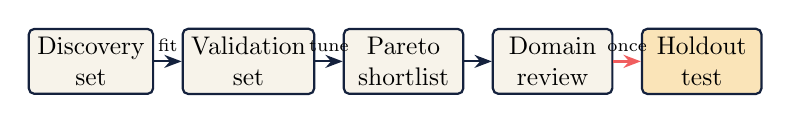
\begin{tikzpicture}[node distance=0.38cm,scale=0.92,transform shape]
    \node[activity] (train) {Discovery\\set};
    \node[activity,right=of train] (valid) {Validation\\set};
    \node[activity,right=of valid] (pareto) {Pareto\\shortlist};
    \node[activity,right=of pareto] (review) {Domain\\review};
    \node[activity,right=of review,fill=Gold!35] (test) {Holdout\\test};
    \draw[flow] (train)--node[above,font=\scriptsize]{fit}(valid);
    \draw[flow] (valid)--node[above,font=\scriptsize]{tune}(pareto);
    \draw[flow] (pareto)--(review);
    \draw[accentflow] (review)--node[above,font=\scriptsize]{once}(test);
  \end{tikzpicture}
  \vspace{0.55cm}
  Report:
  \begin{itemize}
    \item Candidate-generation rules and excluded candidates
    \item Full metric vectors with uncertainty, not only the selected model
    \item Pareto-front membership and the final decision rule
    \item Holdout performance, known instability, and intended model use
  \end{itemize}
\end{frame}

% ===========================================================================
% Unit 8
% ===========================================================================
\lecture{Conformance Checking}{08}
\section{Conformance checking}
\unitdivider{08}{Conformance Checking}
  {Find the smallest meaningful explanation of how reality and the model differ.}

\begin{frame}{What counts as non-conformance?}
  \begin{columns}[T,onlytextwidth]
    \column{0.46\textwidth}
      \textbf{The model may be normative}
      \begin{itemize}
        \item Policy
        \item Regulation
        \item Standard operating procedure
      \end{itemize}
      A deviation may indicate risk.
    \column{0.46\textwidth}
      \textbf{The model may be descriptive}
      \begin{itemize}
        \item Earlier discovery
        \item Expected operating pattern
        \item Simulation baseline
      \end{itemize}
      A deviation may indicate change.
  \end{columns}
  \vspace{0.5cm}
  \keyidea{Conformance identifies differences. Domain context determines whether
  those differences are harmful, helpful, or simply missing from the model.}
\end{frame}

\begin{frame}{Reading an alignment}
  \small
  \begin{tabular}{@{}lccccc@{}}
    \toprule
    Position & 1 & 2 & 3 & 4 & 5\\
    \midrule
    Log & Receive & Check & Clarify & Approve & Ship\\
    Model & Receive & Check & $\gg$ & Approve & Ship\\
    Move & sync & sync & log & sync & sync\\
    \bottomrule
  \end{tabular}
  \vspace{0.55cm}
  \begin{columns}[T,onlytextwidth]
    \column{0.30\textwidth}
      \textbf{Synchronous move}\\Event and model agree.
    \column{0.30\textwidth}
      \textbf{Move on log}\\Observed event not matched.
    \column{0.30\textwidth}
      \textbf{Move on model}\\Expected behavior not observed.
  \end{columns}
\end{frame}

\begin{frame}{From deviations to findings}
  \begin{enumerate}
    \item \textbf{Locate}: Which activities, paths, and cases deviate?
    \item \textbf{Quantify}: How frequent, costly, or delayed are they?
    \item \textbf{Segment}: Which products, teams, or periods differ?
    \item \textbf{Validate}: Is the model current and the data complete?
    \item \textbf{Explain}: What operational mechanism could produce this?
  \end{enumerate}
  \vspace{0.4cm}
  \begin{block}{Strong finding}
    ``Manual credit review is skipped in 7.3\% of high-value orders, concentrated
    in one channel after the April system release.''
  \end{block}
\end{frame}

\begin{frame}[fragile]{Alignment diagnostics in PM4Py}
\begin{lstlisting}[style=python]
alignments = pm4py.conformance_diagnostics_alignments(
    log, net, initial, final
)

for result in alignments[:3]:
    print(result["fitness"])
    print(result["alignment"])
\end{lstlisting}
  \vspace{0.15cm}
  \textbf{Lab output:} a ranked deviation table containing pattern, affected
  cases, frequency, performance impact, and a validated interpretation.
\end{frame}

% ===========================================================================
% Unit 9
% ===========================================================================
\lecture{Performance and Process Enhancement}{09}
\section{Performance enhancement}
\unitdivider{09}{Performance and Process Enhancement}
  {A bottleneck is a mechanism, not merely a red number.}

\begin{frame}{Decompose elapsed time}
  \centering
  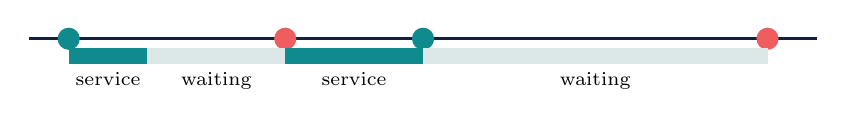
\begin{tikzpicture}[x=1.25cm,y=1cm]
    \draw[very thick,Ink] (0,0)--(8,0);
    \fill[Teal] (0.4,0) circle (4pt);
    \fill[Coral] (2.6,0) circle (4pt);
    \fill[Teal] (4.0,0) circle (4pt);
    \fill[Coral] (7.5,0) circle (4pt);
    \draw[line width=6pt,Teal] (0.4,-0.22)--(1.2,-0.22);
    \draw[line width=6pt,Mist] (1.2,-0.22)--(2.6,-0.22);
    \draw[line width=6pt,Teal] (2.6,-0.22)--(4.0,-0.22);
    \draw[line width=6pt,Mist] (4.0,-0.22)--(7.5,-0.22);
    \node[below,font=\scriptsize] at (0.8,-0.3) {service};
    \node[below,font=\scriptsize] at (1.9,-0.3) {waiting};
    \node[below,font=\scriptsize] at (3.3,-0.3) {service};
    \node[below,font=\scriptsize] at (5.75,-0.3) {waiting};
  \end{tikzpicture}
  \vspace{0.55cm}
  \begin{columns}[T,onlytextwidth]
    \column{0.30\textwidth}\textbf{Throughput time}\\Case start to completion.
    \column{0.30\textwidth}\textbf{Service time}\\Time actively worked.
    \column{0.30\textwidth}\textbf{Waiting time}\\Time between activities.
  \end{columns}
\end{frame}

\begin{frame}{Four bottleneck signatures}
  \begin{columns}[T,onlytextwidth]
    \column{0.47\textwidth}
      \begin{itemize}
        \item Long waiting before one activity
        \item Growing queue over time
        \item Rework returning to the same activity
        \item Excess handovers before completion
      \end{itemize}
    \column{0.47\textwidth}
      \begin{block}{Do not stop at}
        ``Activity X has the longest average duration.''
      \end{block}
      Ask whether the delay comes from capacity, batching, policy, missing
      information, prioritization, or measurement.
  \end{columns}
\end{frame}

\begin{frame}{Compare cohorts, not only averages}
  \small
  \begin{tabular}{@{}lrrr@{}}
    \toprule
    Cohort & Median cycle time & Rework rate & Cases\\
    \midrule
    Standard orders & 2.2 d & 6\% & 4,180\\
    Custom orders & 6.8 d & 29\% & 640\\
    Custom + partner channel & 9.4 d & 41\% & 185\\
    \bottomrule
  \end{tabular}
  \vspace{0.5cm}
  \begin{block}{Improvement hypothesis}
    Partner-channel custom orders arrive with incomplete specifications,
    triggering clarification loops. A structured intake form should reduce
    rework and waiting time.
  \end{block}
  A hypothesis names a mechanism and predicts a measurable change.
\end{frame}

\begin{frame}{From insight to intervention}
  \centering
  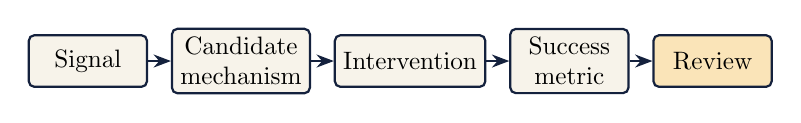
\begin{tikzpicture}[node distance=0.32cm,scale=0.91,transform shape]
    \node[activity] (signal) {Signal};
    \node[activity,right=of signal] (cause) {Candidate\\mechanism};
    \node[activity,right=of cause] (change) {Intervention};
    \node[activity,right=of change] (metric) {Success\\metric};
    \node[activity,right=of metric,fill=Gold!35] (review) {Review};
    \draw[flow] (signal)--(cause);
    \draw[flow] (cause)--(change);
    \draw[flow] (change)--(metric);
    \draw[flow] (metric)--(review);
  \end{tikzpicture}
  \par
  \vspace{0.6cm}
  \keyidea{Process mining supports improvement by narrowing and testing
  explanations. It does not establish causality by itself.}
\end{frame}

% ===========================================================================
% Unit 10
% ===========================================================================
\lecture{Organizational and Multidimensional Analysis}{10}
\section{Organizational analysis}
\unitdivider{10}{Organizational and Multidimensional Analysis}
  {Processes are networks of coordination, not only sequences of activities.}

\begin{frame}{A handover-of-work network}
  \centering
  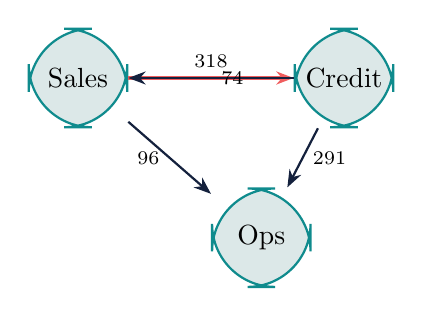
\begin{tikzpicture}[node distance=1.0cm and 2.1cm]
    \node[object,minimum size=1.25cm,rounded corners=8mm] (sales) {Sales};
    \node[object,right=of sales,minimum size=1.25cm,rounded corners=8mm] (credit) {Credit};
    \node[object,below right=0.75cm and 1.05cm of sales,minimum size=1.25cm,rounded corners=8mm] (ops) {Ops};
    \draw[accentflow,bend left=12] (sales)--node[above,font=\scriptsize]{318}(credit);
    \draw[flow,bend left=12] (credit)--node[right,font=\scriptsize]{74}(sales);
    \draw[flow] (credit)--node[right,font=\scriptsize]{291}(ops);
    \draw[flow] (sales)--node[left,font=\scriptsize]{96}(ops);
  \end{tikzpicture}
  \vspace{0.45cm}
  Network analysis can reveal:
  \begin{itemize}
    \item Frequent handovers and coordination loops
    \item Central or overloaded roles
    \item Segregation-of-duties concerns
    \item Differences between formal and actual collaboration
  \end{itemize}
\end{frame}

\begin{frame}{Combine perspectives}
  \begin{columns}[T,onlytextwidth]
    \column{0.22\textwidth}
      \begin{block}{Control flow}
        Which path?
      \end{block}
    \column{0.22\textwidth}
      \begin{block}{Time}
        How long?
      \end{block}
    \column{0.22\textwidth}
      \begin{block}{Organization}
        Who coordinated?
      \end{block}
    \column{0.22\textwidth}
      \begin{block}{Data}
        Under which conditions?
      \end{block}
  \end{columns}
  \vspace{0.55cm}
  \begin{block}{Example synthesis}
    Clarification loops are slowest when cases cross from partner sales to
    central operations, especially for custom products with missing dimensions.
  \end{block}
\end{frame}

\begin{frame}{From an event log to machine-learning rows}
  \centering
  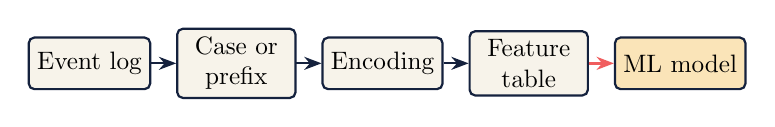
\begin{tikzpicture}[node distance=0.35cm,scale=0.91,transform shape]
    \node[activity] (log) {Event log};
    \node[activity,right=of log] (unit) {Case or\\prefix};
    \node[activity,right=of unit] (encode) {Encoding};
    \node[activity,right=of encode] (features) {Feature\\table};
    \node[activity,right=of features,fill=Gold!35] (ml) {ML model};
    \draw[flow] (log)--(unit);
    \draw[flow] (unit)--(encode);
    \draw[flow] (encode)--(features);
    \draw[accentflow] (features)--(ml);
  \end{tikzpicture}
  \vspace{0.6cm}
  \begin{columns}[T,onlytextwidth]
    \column{0.47\textwidth}
      \textbf{Case-level row}\\One completed case, usually for retrospective
      outcome analysis.
    \column{0.47\textwidth}
      \textbf{Prefix-level row}\\One case observed up to a prediction point,
      used for online monitoring.
  \end{columns}
  \vspace{0.35cm}
  \keyidea{Define the observation cutoff before computing any feature or label.}
\end{frame}

\begin{frame}{Encoding strategies}
  \scriptsize
  \begin{tabular}{@{}
    >{\raggedright\arraybackslash}p{0.18\textwidth}
    >{\raggedright\arraybackslash}p{0.26\textwidth}
    >{\raggedright\arraybackslash}p{0.25\textwidth}
    >{\raggedright\arraybackslash}p{0.215\textwidth}@{}}
    \toprule
    Encoding & Representation & Strength & Main risk\\
    \midrule
    Aggregation & Counts, durations, last value & Simple and strong baseline & Loses order\\
    Index-based & Activity/attribute by position & Preserves early order & Wide, sparse tables\\
    Sequence & Tokens or learned embeddings & Captures order and context & Data and compute demand\\
    Process-aware & Variant, state, alignment moves & Uses domain structure & Model-dependent bias\\
    Graph & DFG/object graph features & Captures relationships & Complex validation\\
    Object-centric & Features by object type & Avoids premature flattening & Aggregation choices remain\\
    \bottomrule
  \end{tabular}
  \vspace{0.45cm}
  \promptbox{Start with an aggregation baseline. Add a richer encoding only when
  it improves validation utility enough to justify complexity.}
\end{frame}

\begin{frame}{Feature provenance is part of the model}
  For every feature, record:
  \begin{itemize}
    \item Source event or object attribute
    \item Aggregation and missing-value rule
    \item Earliest time at which the feature is available
    \item Case/object population to which it applies
    \item Fitted preprocessing parameters and training period
  \end{itemize}
  \vspace{0.35cm}
  \begin{block}{Process-aware examples}
    Rework count, elapsed time, current activity, variant prefix, alignment cost,
    model state, handover count, open-object count, and workload at arrival.
  \end{block}
\end{frame}

\begin{frame}{Responsible resource analysis}
  \begin{itemize}
    \item Analyze roles or teams before individuals where possible
    \item Check workload, case complexity, and data coverage
    \item Avoid ranking people using unvalidated process metrics
    \item Distinguish process constraints from individual performance
    \item Apply access controls, minimization, and purpose limitation
  \end{itemize}
  \vspace{0.45cm}
  \keyidea{Event data reflects the system that assigns work. It is rarely a fair
  standalone measure of an individual's contribution.}
\end{frame}

\begin{frame}{Correlation is a clue, not a cause}
  A team may appear slower because it receives:
  \begin{itemize}
    \item More complex cases
    \item Cases already delayed upstream
    \item Work with poorer data quality
    \item Cases requiring additional controls
  \end{itemize}
  \vspace{0.35cm}
  \promptbox{What additional data or study design would help distinguish a team
  effect from case-mix differences?}
\end{frame}

% ===========================================================================
% Unit 11
% ===========================================================================
\lecture{Object-Centric Process Mining}{11}
\section{Object-centric mining}
\unitdivider{11}{Object-Centric Process Mining}
  {Some processes do not have one natural case identifier.}

\begin{frame}{The flattening problem}
  \begin{columns}[T,onlytextwidth]
    \column{0.46\textwidth}
      \textbf{One order may contain}
      \begin{itemize}
        \item Several items
        \item Several deliveries
        \item Several invoices
        \item One or more payments
      \end{itemize}
    \column{0.48\textwidth}
      \begin{block}{Forced order case}
        Item-level events may be duplicated across the flattened trace.
      \end{block}
      \begin{block}{Forced item case}
        Shared invoice and delivery events may be duplicated instead.
      \end{block}
  \end{columns}
  \vspace{0.4cm}
  This creates \textbf{convergence} and \textbf{divergence}: misleading
  frequencies and apparent behavioral relations.
\end{frame}

\begin{frame}{Object-centric event data}
  \centering
  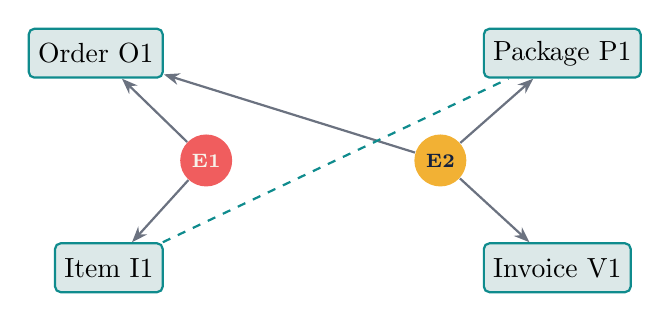
\begin{tikzpicture}[node distance=0.8cm and 1.3cm]
    \node[event] (e1) {E1};
    \node[event,right=2.3cm of e1,fill=Gold,text=Ink] (e2) {E2};
    \node[object,above left=0.8cm and 0.3cm of e1] (order) {Order O1};
    \node[object,below left=0.8cm and 0.3cm of e1] (item) {Item I1};
    \node[object,above right=0.8cm and 0.3cm of e2] (pack) {Package P1};
    \node[object,below right=0.8cm and 0.3cm of e2] (invoice) {Invoice V1};
    \draw[softflow] (e1)--(order);
    \draw[softflow] (e1)--(item);
    \draw[softflow] (e2)--(order);
    \draw[softflow] (e2)--(pack);
    \draw[softflow] (e2)--(invoice);
    \draw[Teal,thick,dashed] (item)--(pack);
  \end{tikzpicture}
  \vspace{0.55cm}
  OCEL 2.0 represents:
  \begin{itemize}
    \item Events linked to one or more typed objects
    \item Object-to-object relationships
    \item Qualified relationships and changing object attributes
  \end{itemize}
\end{frame}

\begin{frame}{Case-centric or object-centric?}
  \small
  \begin{tabular}{@{}p{0.34\textwidth}p{0.28\textwidth}p{0.28\textwidth}@{}}
    \toprule
    Situation & Case-centric & Object-centric\\
    \midrule
    One stable business instance & Strong fit & Often unnecessary\\
    Several interacting entities & Distorting & Strong fit\\
    Established KPI by case & Direct & Requires aggregation choices\\
    Familiar tooling & Mature & Emerging\\
    Relationship questions & Limited & Native\\
    \bottomrule
  \end{tabular}
  \vspace{0.5cm}
  \keyidea{Object-centric analysis does not eliminate modeling choices. It makes
  relationships explicit so those choices are visible.}
\end{frame}

\begin{frame}{Object-centric features without premature flattening}
  \begin{columns}[T,onlytextwidth]
    \column{0.47\textwidth}
      \textbf{Per object type}
      \begin{itemize}
        \item Counts and lifecycle states
        \item Age and elapsed-time summaries
        \item Completed and open related objects
        \item Relationship cardinalities
      \end{itemize}
    \column{0.47\textwidth}
      \textbf{At prediction time}
      \begin{itemize}
        \item Freeze the object graph at the cutoff
        \item Aggregate only visible objects
        \item Preserve identifiers for grouped splits
        \item Test sensitivity to aggregation rules
      \end{itemize}
  \end{columns}
  \vspace{0.45cm}
  \keyidea{Flatten late and explicitly. The target object and prediction time
  should determine which relationships become features.}
\end{frame}

\begin{frame}[fragile]{Inspect an OCEL with PM4Py}
\begin{lstlisting}[style=python]
import pm4py

ocel = pm4py.read_ocel2_json("order_management.jsonocel")

print(ocel.events.head())
print(ocel.objects.head())
print(ocel.relations.head())

ocdfg = pm4py.discover_ocdfg(ocel)
pm4py.save_vis_ocdfg(ocdfg, "object_centric.svg")
\end{lstlisting}
  \vspace{0.15cm}
  \textbf{Lab comparison:} flatten the same data by order and by item. Which
  frequencies or paths become misleading?
\end{frame}

% ===========================================================================
% Unit 12
% ===========================================================================
\lecture{Process-Mining Projects and Communication}{12}
\section{Projects and communication}
\unitdivider{12}{Projects and Communication}
  {A process-mining project succeeds when evidence changes a decision.}

\begin{frame}{The project lifecycle}
  \centering
  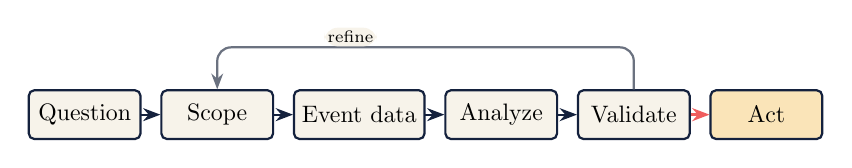
\begin{tikzpicture}[node distance=0.28cm,scale=0.86,transform shape]
    \node[activity] (q) {Question};
    \node[activity,right=of q] (scope) {Scope};
    \node[activity,right=of scope] (data) {Event data};
    \node[activity,right=of data] (analyse) {Analyze};
    \node[activity,right=of analyse] (validate) {Validate};
    \node[activity,right=of validate,fill=Gold!35] (act) {Act};
    \draw[flow] (q)--(scope);
    \draw[flow] (scope)--(data);
    \draw[flow] (data)--(analyse);
    \draw[flow] (analyse)--(validate);
    \draw[accentflow] (validate)--(act);
    \draw[softflow,rounded corners=5pt]
      (validate.north) -- ++(0,0.62)
      -| node[pos=0.34,above,font=\scriptsize,fill=Paper,inner sep=1.5pt]
        {refine}
      (scope.north);
  \end{tikzpicture}
  \par
  \vspace{0.6cm}
  The lifecycle is iterative. Domain validation may change the event mapping,
  case notion, model, metric, or even the original question.
\end{frame}

\begin{frame}{Predictive process monitoring tasks}
  \small
  \begin{tabular}{@{}
    >{\raggedright\arraybackslash}p{0.22\textwidth}
    >{\raggedright\arraybackslash}p{0.24\textwidth}
    >{\raggedright\arraybackslash}p{0.25\textwidth}
    >{\raggedright\arraybackslash}p{0.195\textwidth}@{}}
    \toprule
    Question & ML formulation & Example target & Useful baseline\\
    \midrule
    What happens next? & Classification & Next activity & Most frequent transition\\
    How long remains? & Regression / survival & Remaining time & Median by current state\\
    How will it end? & Classification & Late / rejected / compliant & Base-rate model\\
    Is this unusual? & Anomaly detection & Deviant prefix & Frequency / conformance score\\
    \bottomrule
  \end{tabular}
  \vspace{0.45cm}
  \keyidea{The prediction must correspond to an operational decision and a time
  when someone can still act.}
\end{frame}

\begin{frame}{Prefixes, labels, and prediction points}
  \centering
  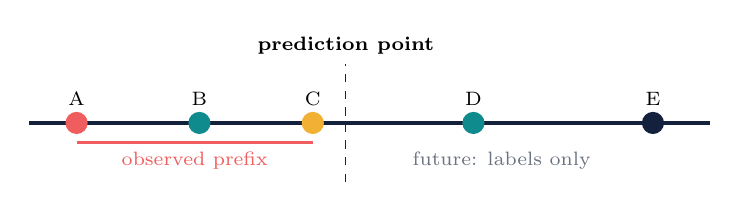
\begin{tikzpicture}[x=1.2cm,y=1cm]
    \draw[very thick,Ink] (0,0)--(7.2,0);
    \foreach \x/\lab/\col in {
      0.5/A/Coral,1.8/B/Teal,3.0/C/Gold,4.7/D/Teal,6.6/E/Ink}
      {
        \fill[\col] (\x,0) circle (4pt);
        \node[above,font=\scriptsize] at (\x,0.10) {\lab};
      }
    \draw[very thick,Coral] (0.5,-0.25)--(3.0,-0.25);
    \draw[dashed,Ink] (3.35,-0.75)--(3.35,0.75);
    \node[below,text=Coral,font=\scriptsize] at (1.75,-0.25)
      {observed prefix};
    \node[above,font=\scriptsize\bfseries] at (3.35,0.75)
      {prediction point};
    \node[below,text=SoftGray,font=\scriptsize] at (5.0,-0.25)
      {future: labels only};
  \end{tikzpicture}
  \vspace{0.55cm}
  \begin{columns}[T,onlytextwidth]
    \column{0.47\textwidth}
      \textbf{Define}
      \begin{itemize}
        \item Prefix rule and cutoff
        \item Prediction frequency
        \item Label horizon
      \end{itemize}
    \column{0.47\textwidth}
      \textbf{Avoid}
      \begin{itemize}
        \item Features computed after cutoff
        \item Labels unavailable in operation
        \item Duplicated prefixes across splits
      \end{itemize}
  \end{columns}
\end{frame}

\begin{frame}{Split by time, group by case}
  \centering
  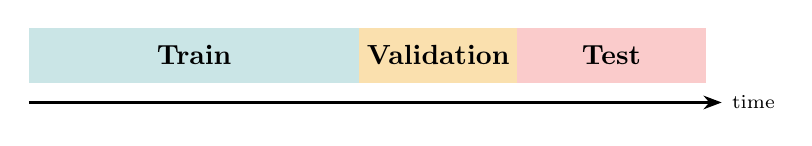
\begin{tikzpicture}[x=1cm,y=1cm]
    \fill[Teal!22] (0,0) rectangle (4.2,0.7);
    \fill[Gold!40] (4.2,0) rectangle (6.2,0.7);
    \fill[Coral!32] (6.2,0) rectangle (8.6,0.7);
    \node at (2.1,0.35) {\textbf{Train}};
    \node at (5.2,0.35) {\textbf{Validation}};
    \node at (7.4,0.35) {\textbf{Test}};
    \draw[-{Stealth},thick] (0,-0.25)--(8.8,-0.25)
      node[right,font=\scriptsize]{time};
  \end{tikzpicture}
  \vspace{0.45cm}
  \begin{itemize}
    \item Assign every case and all its prefixes to exactly one split.
    \item Fit encoders, imputers, scalers, and vocabularies on training data only.
    \item Prefer temporal evaluation when the deployed model predicts future cases.
    \item Keep related customers, orders, or objects together when dependence exists.
    \item Reserve the test period for one final estimate after tuning.
  \end{itemize}
\end{frame}

\begin{frame}{Common leakage paths}
  \begin{columns}[T,onlytextwidth]
    \column{0.47\textwidth}
      \textbf{Future leakage}
      \begin{itemize}
        \item Final case attributes in a prefix
        \item Total event count or final duration
        \item Post-outcome resource or status
      \end{itemize}
      \textbf{Split leakage}
      \begin{itemize}
        \item Prefixes from one case in several splits
        \item Random event-level splitting
      \end{itemize}
    \column{0.47\textwidth}
      \textbf{Preprocessing leakage}
      \begin{itemize}
        \item Global normalization or imputation
        \item Variants built from all periods
        \item Discovery model fitted on test cases
      \end{itemize}
      \textbf{Operational leakage}
      \begin{itemize}
        \item Feature not available at scoring time
        \item Label definition changes after deployment
      \end{itemize}
  \end{columns}
\end{frame}

\begin{frame}{Evaluate beyond predictive accuracy}
  \begin{columns}[T,onlytextwidth]
    \column{0.22\textwidth}
      \begin{block}{Discrimination}
        AUC, PR-AUC, MAE, concordance
      \end{block}
    \column{0.22\textwidth}
      \begin{block}{Calibration}
        Reliability, Brier score, interval coverage
      \end{block}
    \column{0.22\textwidth}
      \begin{block}{Timeliness}
        Earliness, stability across prefixes
      \end{block}
    \column{0.22\textwidth}
      \begin{block}{Utility}
        Cost, workload, prevented delay, decision value
      \end{block}
  \end{columns}
  \vspace{0.5cm}
  Also monitor:
  \begin{itemize}
    \item Performance by cohort and process state
    \item Feature, label, and process drift
    \item Alert volume, false-alarm burden, and intervention capacity
  \end{itemize}
\end{frame}

\begin{frame}{Integration patterns: process mining + ML}
  \small
  \begin{columns}[T,onlytextwidth]
    \column{0.47\textwidth}
      \begin{block}{Process mining informs ML}
        Variants, model state, alignments, conformance, rework, and handovers
        become features or cohorts.
      \end{block}
      \begin{block}{ML informs process analysis}
        Predictions identify risky prefixes and reveal where errors concentrate
        in the process.
      \end{block}
    \column{0.47\textwidth}
      \centering
      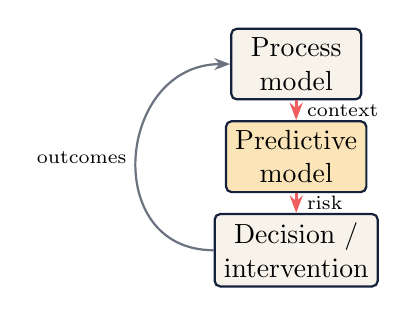
\begin{tikzpicture}[node distance=0.25cm]
        \node[activity] (pm) {Process\\model};
        \node[activity,below=of pm,fill=Gold!35] (ml) {Predictive\\model};
        \node[activity,below=of ml] (action) {Decision /\\intervention};
        \draw[accentflow] (pm)--node[right,font=\scriptsize]{context}(ml);
        \draw[accentflow] (ml)--node[right,font=\scriptsize]{risk}(action);
        \draw[softflow] (action.west)
          to[out=180,in=180,looseness=1.55]
          node[left,font=\scriptsize]{outcomes}(pm.west);
      \end{tikzpicture}
  \end{columns}
  \vspace{0.1cm}
  \keyidea{Version and monitor the event mapping, process model, encoding, and
  predictive model as one analytical system.}
\end{frame}

\begin{frame}{An evidence chain for every finding}
  \begin{enumerate}
    \item \textbf{Question}: what decision is at stake?
    \item \textbf{Observation}: what pattern is measured?
    \item \textbf{Interpretation}: what mechanism may explain it?
    \item \textbf{Validation}: what did domain experts or other data confirm?
    \item \textbf{Action}: what change should be tested?
    \item \textbf{Metric}: how will we know whether it worked?
  \end{enumerate}
  \vspace{0.35cm}
  \keyidea{Separate observation from interpretation. It makes the analysis easier
  to challenge, improve, and trust.}
\end{frame}

\begin{frame}{Communicate one finding well}
  \begin{columns}[T,onlytextwidth]
    \column{0.46\textwidth}
      \textbf{Lead with}
      \begin{itemize}
        \item Operational consequence
        \item Magnitude and affected population
        \item Concise visual evidence
        \item Recommended next action
      \end{itemize}
    \column{0.46\textwidth}
      \textbf{Always include}
      \begin{itemize}
        \item Data scope
        \item Key assumptions
        \item Uncertainty
        \item Important alternatives
      \end{itemize}
  \end{columns}
  \vspace{0.45cm}
  \begin{block}{Headline pattern}
    \alert{What happens} + \alert{where} + \alert{impact}: ``Clarification loops
    add 4.1 days to partner-channel custom orders.''
  \end{block}
\end{frame}

\begin{frame}{Reproducibility checklist}
  \begin{columns}[T,onlytextwidth]
    \column{0.47\textwidth}
      \begin{itemize}
        \item Versioned extraction and transformation code
        \item Data dictionary and event semantics
        \item Fixed parameters and package versions
        \item Deterministic figures and tables
      \end{itemize}
    \column{0.47\textwidth}
      \begin{itemize}
        \item Documented exclusions and filters
        \item Stored model artifacts
        \item Decision and validation log
        \item Privacy-aware sharing strategy
      \end{itemize}
  \end{columns}
  \vspace{0.5cm}
  \promptbox{Could another analyst reproduce your central finding without asking
  what you clicked?}
\end{frame}

\begin{frame}{Research opportunities}
  \small
  \begin{columns}[T,onlytextwidth]
    \column{0.47\textwidth}
      \textbf{Richer event data}
      \begin{itemize}
        \item Multimodal event logs
        \item Automated event abstraction
        \item Object-centric, streaming, and uncertain events
      \end{itemize}
    \column{0.47\textwidth}
      \textbf{Richer analysis}
      \begin{itemize}
        \item Multimodal representation learning
        \item Causal process mining
        \item Prescriptive monitoring
        \item Privacy-preserving analytics
      \end{itemize}
  \end{columns}
  \vspace{0.15cm}
  \begin{block}{Multimodal event logs}
    Align structured events with payload such as free text, documents, images,
    audio, and sensor streams while preserving time, provenance, and access rules.
  \end{block}
  \vspace{0.05cm}
  \keyidea{Each modality must add valid, timely, and governable process evidence.}
\end{frame}

% ===========================================================================
% Capstone and close
% ===========================================================================
\lecture{Capstone and course close}{13}
\section{Capstone}

\begin{frame}{Capstone: end-to-end process study}
  \begin{columns}[T,onlytextwidth]
    \column{0.48\textwidth}
      \textbf{Required analysis}
      \begin{itemize}
        \item Scope and analytical questions
        \item Event semantics and quality report
        \item Representation, flattening, and encoding
        \item Exploration, performance, and discovery
        \item Quality vector and Pareto-front comparison
        \item Conformance or deviation analysis
      \end{itemize}
    \column{0.48\textwidth}
      \textbf{Required argument}
      \begin{itemize}
        \item One validated finding
        \item Predictive baseline when relevant
        \item Leakage-safe split and evaluation
        \item One improvement hypothesis
        \item Ethical and analytical limitations
        \item Reproducible code and artifacts
        \item Stakeholder-oriented presentation
      \end{itemize}
  \end{columns}
\end{frame}

\begin{frame}{Capstone evaluation}
  \small
  \begin{tabular}{@{}p{0.30\textwidth}p{0.58\textwidth}@{}}
    \toprule
    Dimension & Evidence of strong work\\
    \midrule
    Question and scope & Specific decision, coherent case notion, explicit boundaries\\
    Representation & Validated semantics, justified flattening and encoding\\
    Model quality & Full metric vectors, Pareto analysis, stable selection rule\\
    Prediction & Leakage-safe split, calibrated errors, operational baseline\\
    Interpretation & Findings distinguish evidence from explanation\\
    Reproducibility & Analysis runs from documented inputs to outputs\\
    Communication & Consequence, uncertainty, and next action are clear\\
    \bottomrule
  \end{tabular}
\end{frame}

\begin{frame}{The analyst's discipline}
  \Large
  \begin{enumerate}
    \item Question the event semantics.
    \item Make representation choices explicit.
    \item Compare quality vectors, not one score.
    \item Prevent leakage before training.
    \item Turn findings and predictions into testable actions.
  \end{enumerate}
  \vspace{0.35cm}
  \keyidea{The most important process-mining skill is knowing what the data can
  support you in saying.}
\end{frame}

\begin{frame}[plain]
  \begin{tikzpicture}[remember picture,overlay]
    \fill[DeepInk] (current page.south west) rectangle (current page.north east);
    \fill[Coral] (current page.south west) rectangle
      ([yshift=0.13\paperheight]current page.south east);
    \node[text=Paper,font=\fontsize{31}{34}\selectfont\bfseries]
      at ([yshift=0.55cm]current page.center) {Questions become evidence.};
    \node[text=Mist,font=\Large]
      at ([yshift=-0.75cm]current page.center) {Evidence becomes better process decisions.};
    \node[text=Paper,font=\small]
      at ([yshift=0.065\paperheight]current page.south) {\coursename\quad|\quad\instructor};
  \end{tikzpicture}
\end{frame}

% ===========================================================================
% References
% ===========================================================================
\section{References}

\begin{frame}{References — core textbook}
  \begin{block}{Main reference}
    van der Aalst, W.M.P. (2016). \textit{Process Mining: Data Science in
    Action} (2nd ed.). Springer.
  \end{block}
  \vspace{0.4cm}
  This textbook, by the founder of the process mining field, is the primary
  reference for the concepts covered throughout the course: event log
  semantics, process discovery, conformance checking, and process
  enhancement.
\end{frame}

\begin{frame}[shrink=8]{References — selected articles}
  \small
  \begin{enumerate}
    \item de Alvarenga, S.C., Barbon Jr., S., Miani, R.S., Cukier, M.,
      Zarpelão, B.B. (2018). Process mining and hierarchical clustering to
      help intrusion alert visualization. \textit{Computers \& Security},
      73, 474--491.
      \url{https://www.sciencedirect.com/science/article/pii/S0167404817302584}

    \item Ceravolo, P., Tavares, G.M., Barbon Jr., S., Damiani, E. (2020).
      Evaluation Goals for Online Process Mining: A Concept Drift
      Perspective. \textit{IEEE Transactions on Services Computing}.
      \url{https://ieeexplore.ieee.org/abstract/document/9124702}

    \item Tavares, G.M., Oyamada, R.S., Barbon Jr., S., Ceravolo, P.
      (2023). Trace encoding in process mining: A survey and benchmarking.
      \textit{Engineering Applications of Artificial Intelligence}, 126,
      107028.
      \url{https://www.sciencedirect.com/science/article/pii/S0952197623012125}

    \item da Silva, M.C., Tavares, G.M., Gritti, M.C., Ceravolo, P.
      (2023). Using Process Mining to Reduce Fraud in Digital Onboarding.
      \textit{FinTech}, 2(1), 120--137.
      \url{https://www.mdpi.com/2674-1032/2/1/9}
  \end{enumerate}
\end{frame}

\end{document}
